% !TEX root = ../thesis-example.tex
%
\chapter{L'instrument et le geste}
\label{ch:gesture}

\cleanchapterquote{La percussion de ce pseudo-gong est illlusoire :\\
rien ne tape sur rien dans l’ordinateur.\\
Schumann qualifiait le legato au piano\\
de ``trompe-l’oreille'' : la musique est aussi un art\\
du mirage, de l’illusion.}{Jean-Claude Risset}{Discours invité aux JIM 2010 \cite{risset_propos_2010}}

Proprioception et schema corporels (cf. Miranda unconventional computing)

%L'expression musicale a été contrainte (et non ``prisonnière'', car la contrainte peut être fertile) par la relation causale entre le geste d'excitation et le son produit par l'instrument dans les lutheries acoustiques.

\noindent Poursuivant des évolutions organologiques latentes, telles que présentées dans la section \ref{sec:ephemerality:landscape}, les \glspl{DMI} finissent d'opérer un découplage énergétique, une ``dislocation du contrôle'' (\textit{control dislocation} \cite{miranda_new_2006}), rompant avec plus de 35.000 ans de tradition musicale \cite{conard_new_2009} et avec l'unité de temps, de lieu et d'action —définie en règle par le théâtre classique, mais qui reflète la relation qui existait entre l'auditeur et le phénomène sonore, comme le rappelle Hugues Genevois dans \cite{cance_what_2012}.\\
\indent L'introduction de la mémoire et de la computation numérique permet une re-programmation complète de l'interaction, rendant leur fonctionnement à la fois complexe et cryptique. Cet aspect peut se révéler être un inconvénient, dans la mesure où il prive le public d’une lecture possible de la performance musicale. Cela peut cependant s’avérer être un avantage, si l'on considère que la performance musicale comporte une part scénographique dans laquelle l’illusion a toute sa place.\\
\indent Nous allons voir dans ce chapitre comment le geste instrumental s'en trouve affecté, par un examen critique des catégories gestuelles déjà proposées, la proposition de nouvelles catégories prenant en compte l'aspect subversif de l'art musical et les conséquences que nous pouvons en tirer en termes de conceptions des \glspl{DMI}.


\section{Introduction : L'étude du geste en musique}

\noindent Si l'étude du rythme et plus encore, des hauteurs, a été particulièrement importante dans la culture classique occidentale, l'étude du geste a longtemps été négligée voire méprisée, comme le rapporte Jean-Marc Warszawski\footnote{Conférence La musique et le geste : \url{https://www.musicologie.org/18/la_musique_et_le_geste.html}.}: \iquote{La tradition savante occidentale, grâce à l'écriture, dématérialise le geste créatif musicien, et impose une ligne de démarcation ente musique écrite et non écrite, en quelque sorte une frontière entre le primitif et le civilisé.}\\
\indent Peut-être faut-il également y voir une autre raison : le geste ne se laisse pas aussi facilement mesurer, encore moins définir, que la hauteur. Si cette dernière peut se  réduire en première approximation à une grandeur physique mesurable --~sa fréquence\footnote{La perception de la hauteur est évidemment plus complexe et un des sujets d'étude de la psycho-acoustique, voir notamment les travaux de Michèle Castellengo \cite{castellengo_ecoute_2015}. L'écriture musicale classique s'est toutefois largement construite sur cette réduction, que Robert Francès nomme ``abstraction notale'' \cite{frances_perception_1984}.}, le geste ne se laisse pas aussi facilement réduire à une mesure. Il entraine depuis sa production jusqu'à sa réception toute la complexité du vivant : sa multidimensionalité, son instabilité, sa relativité, sa combinatoire, et l'ensemble de ses aspects culturels... (TODO : développer et/ou enlever les pointillés)\\
\indent L'étude du geste se développe dans le courant du \siecle{19}~siècle, sous l'effet de la révolution industrielle, de l'étude mécanique du mouvement et la création de conservatoires qui développent des techniques d'apprentissage où le geste est pris en compte\footnote{Voir en particulier la collection rassemblée sur le site de la Bibliothèque Nationale de France: \url{https://gallica.bnf.fr/html/und/partitions/oeuvres-theoriques-et-pedagogiques}. L'intérêt pour le geste à cette période de développement industriel donne lieu par ailleurs à l'invention d'étonnants systèmes mécaniques servant à guider, contraindre et fortifier les gestes, en particulier pour le piano, tels que le ``chiroplaste'' ou le ``dactylion'', mais qui s'avèrent être davantage des instruments de torture, endommageant parfois les mains de manière irréversible.}. L'étude du geste a progressivement gagné en importance, d'une part avec l'émergence de l'anthropologie au début du \siecle{20}~siècle, et d'autre part suite à l'explosion des technologies de télécommunication, lorsque sa compréhension et sa modélisation sont devenues nécessaires pour le développement des \gls{IHM} dans la seconde moitié du siècle, jusqu'à devenir un domaine d'étude à part entière, les \textit{gesture studies}, soutenue notamment par l'\gls{ISGS} créée en 2002.\\
\indent Dans le domaine de la musique, c'est l'arrivée du ``temps-réel'' et l'émergence des \glspl{DMI} dans les années 1980, qui entraine la parution croissante d'articles traitant de la question du geste instrumental. Au tournant du siècle (du millénaire), le geste devient un objet d'étude majeur dans le domaine de l'informatique musicale, se traduisant notamment par la parution d'ouvrages collectifs dédiés\footnote{Voir en particulier : \cite{genevois_les_1999}, \cite{wanderley_trends_2000} et \cite{godoy_musical_2010}}, ainsi par que l'apparition de la conférence \gls{NIME} en 2001, qui lui accorde une place importante.\\
\indent Plusieurs projets de recherche interdisciplinaires ont également été menés, comme le projet ConGAS\footnote{``Gesture Controlled Audio Systems'', projet financé entre 2003 et 2007 dans le cadre de la Coopération Européenne en Sciences et Technologies (COST Action 287)}, ou plus récemment le projet Gemme\footnote{``Geste musical : modèles et expériences'', projet de recherche financé par l'ANR de 2012 à 2016, dont un carnet de recherche en ligne est disponible : \url{https://geste.hypotheses.org/gemme}} et la chaire thématique pluridisciplinaire GeAcMus\footnote{La chaire``Geste - Acoustique - Musique'' a été créée en 2015 à Sorbonne Université \url{http://www.sorbonne-universites.fr/actions/recherche/chaires-thematiques/geacmus.html}} créée à Sorbonne-Université.

\extra{Le terme Gesture est utilisé dans 62\% des articles publiés à NIME (cf. Jensenius paper : To Gesture or Not? An Analysis of Terminology in NIME Proceedings 2001–2013) <= update this}


\section{Geste instrumental et geste musical}

\subsection{La musique et ses instruments}

\noindent La définition du geste musical pose le double problème de définir ce qu'on entend par ``geste'' et par ``musique''. Pour ce qui est de la musique, j'adopterai ici la définition proposée par Christopher Small, non pas du \textit{nom} ``musique'', mais du \textit{verbe} qu'il invente : ``musiquer'' \cite{small_musicking:_1998}:
\iquote{Musiquer, c'est participer, à quelque titre que ce soit, à une performance musicale, que ce soit en jouant, en écoutant, en répétant ou en pratiquant, en fournissant du matériel pour la performance (ce qu'on appelle ``composer''), ou en dansant. Nous pourrions même parfois en étendre le sens à ce que font la personne qui prend les billets à l'entrée, les gros bras qui déplacent le piano et les tambours, les roadies qui installent les instruments et font les balances ou les personnes qui nettoient après que tout le monde soit parti. Ils contribuent tous, eux aussi, à la nature de l'événement qu'est une performance musicale.}\\
\indent Si j'adopte ce néologisme, ce n'est pas pour l'exhaustivité que semble conférer une définition aussi large mais essentiellement pour deux raisons: la première est le choix d'utiliser un verbe plutôt qu'un nom, c'est-à-dire d'identifier une pratique plutôt qu'un objet, ce qui dans le cas de la performance musicale semble mieux adapté. La deuxième raison est liée au contexte technico-culturel dans lequel ces pratiques s'inscrivent: la reconfiguration des modes de production et de réception de la musique\footnote{voir à ce sujet l'ouvrage de Paul Théberge \cite{theberge_any_1997}} qu'ont entrainée les évolutions technologiques du \siecle{20}~siècle ont rendu poreuses les frontières entre les différentes pratiques liées à la création musicale. Je restreindrai toutefois le champ de cette définition aux pratiques qui gravitent directement autour de l'instrument de musique, tel que présenté dans le chapitre précédent.\\
\indent Partant de cette définition et reprenant une proposition d'Hugues Genevois \cite{genevois_geste_1999}, on peut distinguer plusieurs phases au cours desquelles se manifeste un geste musical :

\vspace{-1em}
\begin{itemize}[noitemsep]
\item \textbf{la composition} : la production de structure musicales hors-temps de leur rendu sonore;
\item \textbf{la lutherie} : la réalisation de l'instrument et sa préparation pour le jeu;
\item \textbf{la performance} : le jeu instrumental qui produit, modifie, mélange, dans le temps même de l'écoute, la matière sonore, les gestes de l'instrumentiste, du chef, de l'ingénieur du son;
\item \textbf{l'écoute} : qui construit l'intelligibilité de notre environnement sonore et se mobilise sans répit pour en garantir la cohérence;
\item \textbf{la pédagogie} : durant laquelle la complexité du geste musical se transmet progressivement, en étant guidée, soutenue, encouragée, critiquée, en se pratiquant parfois sous la forme d'exercices idiomatiques et systématiques (e.g. faire ses gammes), et à travers des allers-retours entre performance et écoute.
\end{itemize}

\noindent Dans la pratique, ces différents gestes se superposent souvent mais pourront se traduire par différentes formes de configurations instrumentales, adaptées aux spécificités de chaque situation (TODO : développer ou renvoyer à une section ultérieure qui développe).

\subsection{Définition(s) du geste}

\noindent Dans sa définition générale, le Littré, le Larousse ou le dictionnaire de l'Académie Française s'accordent à le définir comme \iquote{un mouvement du corps, principalement de la main, des bras, de la tête, porteur de sens ou non} (Larousse).

\noindent \textbf{aspect phénoménologique} Un premier aspect du geste est sa nature en mouvement, son déploiement spatial et temporel. En soi, le geste possède des qualités de mouvements, en dehors de toute interprétation. Ce mouvement est l'expression même du vivant et il reflète à la fois la relation du corps à son environnement externe (force de gravité et cinétique, contournement d'obstacles, frictions sur les matériaux...) et l'expression des mouvements internes du corps (vigueur ou mollesse, souple ou crispé, émotion se traduisant par des gestes tels que haussement d'épaule, sursaut de surprise, grimaces diverses, etc.). La maitrise de ces mouvements est un aspect fondamental de la danse qui, comme la musique le fait avec le son, met en œuvre le corps dans des intensités, des rythmes, des trajectoires. Si les gestes de la danse ne sont pas \textit{a priori} instrumentaux, les \glspl{DMI} rendent plus que jamais possible leur utilisation à des fins d'interaction musicale, comme nous le verrons plus loin (cf. notamment \cite{bevilacqua_gesture_2011, alaoui_movement_2012, silang_maranan_designing_2014, hsueh_understanding_2019}.)

\noindent \textbf{aspect sémiotique} Un deuxième aspect du geste est indiqué par le curieux épithète de la définition précédente : ``porteur de sens ou non''. S'il a semblé utile d'évoquer une qualité potentiellement absente, c'est précisément parce les différentes définitions qu'on donne du geste dépendent en partie de cet aspect sémiotique, qui reste soumis à une interprétation subjective et contextuelle dans un système de valeurs. Les significations d'un geste peuvent en effet être attribuées par l'auteur du geste ou bien par celui ou celle qui observe ce geste, sans qu'il n'y ait nécessairement de correspondance, ni en terme de signification, ni sur la part du mouvement considérée signifiante. La signification d'un geste peut également être attribuée par la machine, en particulier dans les systèmes d'apprentissage, comme nous le verrons plus loin.

\noindent \textbf{aspect ergotique} Une autre définition du geste relève sa dimension manipulative : \iquote{Manière de mouvoir le corps, les membres et, en particulier, manière de mouvoir les mains dans un but de préhension, de manipulation} (Larousse). Cette définition met l'accent sur la relation possible entre le geste et un objet, un outil, un instrument et s'applique par conséquence particulièrement bien à la situation instrumentale. C'est sur cet aspect que se concentre notamment les typologies gestuelles proposées par Claude Cadoz que nous discuterons plus loin.

\noindent \textbf{aspect (dia)grammatique} Enfin, si le geste \textit{ex-prime} (du latin \textit{ex-premo} : ``faire sortir en pressant'') des mouvements internes du corps, qu'ils soient d'origine émotionnelle, sémiotique ou simplement dynamique, le geste \textit{im-prime} et laisse une trace dans la matière, dans la machine, dans les esprits. C'est parfois cette trace résultante qu'on nomme geste, par métonymie et analogie avec les qualités de mouvement qui sont à son origine, lorsqu'on parle par exemple du \textit{geste de composition}. Les capacités des machines à enregistrer le geste dans sa dynamique --~auparavant éphémère et seulement visible dans sa trace~-- confèrent à ce sens particulier du geste une importance particulière \iquote{à l'époque de sa reproductibilité technique}\cite{benjamin_loeuvre_2013}, qu'il nous faut souligner et qui sera analysée en dernier lieu.


La fonction sémiotique du geste a occupé une grande place dans son étude au \siecle{20}~siècle, notamment sous l'influence conjointe de l'anthropologie naissante, analysant les systèmes d'interaction sociale de différentes cultures \footnote{Adam Kendon, Marcel Jousse, Bernard Koechlin, André Leroi-Gourhan...} mais aussi de l'explosion de la télécommunication et des recherches scientifiques qui ont accompagné cette révolution technologique.

L'influence de la théorie de l'information de Claude Shannon (cf. figure TODO), en particulier, a contribué à envisager le geste, dans une perspective communicationnelle. Les analyses qui en résultent s'inscrivaient alors, plus ou moins explicitement, dans une perspective d'encodage efficace, en extrayant l'information qu'il contient, et par inférence, sa signification supposée.

Cette influence est particulièrement sensible dans l'école Anglo-Saxonne, centrée sur les figures de Adam Kendon et David McNeil, qui confèrent au geste une signification préalable à son existence. D'après McNeil, \iquote{(...) le geste est créé par le locuteur comme une matérialisation du sens'' \iquote{(...) a gesture does not represent at all; the gesture is created by the speaker as a materialization of meaning. }, \cite{mcneill_gesture_2005}}

A l'opposé, l'approche phénoménologique adopte un autre point de vue en conférant au geste un statut pré-sémiotique et un pouvoir créatif et expressif.
Guerino Mazzola : \iquote{Gestures are dialogical, live in presence, are circular, elastic, are presemiotic, and are as such already differentiated (being gestural can be ramified into different types).} \cite{mazzola_topos_2018}, p. 59 (852)

Le geste peut être porteur d'un sens préalable (McNeil) ou d'un sens 

D'une certaine manière, ces deux approches se placent de part et d'autre du processus de communication, du point de vue de l'auteur du geste (Gesture and thoughts, chez McNeil) et de son observateur (Phénoménologie de la perception).

Le geste \textit{exprime} (du latin \textit{ex-premo} : ``faire sortir en pressant'') quelque chose, mais n'a pas nécessairement une signification.


Pour autant, on se rend bien compte que tous les mouvements du corps ne sont pas nécessairement en permanence associés à l'idée de geste. Dans le cadre d'une activité spécifique telle que la pratique musicale, impliquant la participation active de l'individu, la plupart des études (todo:mettre plusieurs ref) sur le geste s'accordent à le définir comme l'association d'un mouvement et d'une intention.

\iquote{Le geste doit être défini comme un mouvement intentionnel plus ou moins complexe, orienté vers un but déterminé qui lui donne un sens individuel, social ou historique.} \cite{imberty_mouvement_2013}

\noindent L'intention gestuelle peut être envisagée selon différent points de vue, selon que son étude porte sur sa fonction sémiotique (le geste-signe), ergotique (le geste-action), épistémique (le geste de perception).\\
\indent La notion de geste est également utilisée pour décrire des formes indirectement liées au mouvement physique, telles que le ``geste de composition'', en transposant par analogie le mouvement et l'intention le caractérisant. On voit donc que la question de l'intention soulève des questions esthétiques voire politiques : l'inscription de la performance musicale dans la vie sociale et culturelle pose la question de la place du geste dans un système de valeurs spécifique. En particulier, l'époque postmoderne est caractérisée par un art qui attribue davantage d'importance à \textit{l'intérêt} du geste pris dans un contexte \textit{expérimental}, qu'à sa \textit{beauté}, prise dans un contexte \textit{normatif} classique.

\indent Enfin, en tant que phénomène de transfert d'énergie et d'information, le geste pourra être évaluée différemment selon qu'on se place du point de vue de sa production ou de celui de sa réception. 

La ``geste'' en musique a ainsi été utilisée pour décrire différents aspects de la relation qu'entretiennent le mouvement, l'instrument, l'intention, la morphologie et la signification du son ou encore les formes d'écritures compositionnelles. L'instrument de musique se trouvant à la croisée de ces différents chemins, la notion de ``geste instrumental'' a souvent été liée voire confondue avec celle de ``geste musical''. 

La relation entre musique et mouvement du corps dépasse le domaine de l'interaction instrumentale. Par exemple, les mouvements de la danse, s'il peuvent être en corrélation avec la musique, ne sont pas a priori des gestes instrumentaux. Cependant, si les mouvements du danseur sont captés et interagissent avec la production du son — ce qui est particulièrement rendu possible avec les nouvelles technologies, alors ils peuvent être envisagés comme relevant du geste instrumental.

Le geste instrumental parait au premier abord plus simple que le geste musical, en ce qu'il semble davantage possible de le décrire à travers une approche purement fonctionnelle de sa mécanique. 

Dès 1995, Todd Winkler propose de repenser le geste instrumental dans les \glspl{DMI} en proposant des contraintes et des idiomes libérés du modèle de l'instrument acoustique \cite{winkler_making_1995}. Sa formulation de cette problématique est intéressante en ce qu'elle envisage déjà la sonorité des gestes au-delà du modèle acoustique excitation/résonance (``le son du claquement d'une seule main''). Cependant, ses propositions reflètent son attachement au paradigme physique et à la corrélation entre l'énergie du geste et du son : \iquote{Qu'est ce que la musique des doigts ? Qu'est ce que la musique de course ? Quel \textit{est} le son d'\textit{une seule} main qui claque ? On peut répondre à ces questions en permettant à la physicalité du mouvement d'avoir un impact sur le matériel et les processus musicaux. Ces relations peuvent être établies en considérant le corps et l'espace comme des instruments de musique, libérés des relations dans les instruments acoustiques, mais avec des contraintes similaires qui peuvent donner du caractère au son par des mouvements idiomatiques.}\footnote{\iquote{What is finger music? What is running music? What \textit{is} the sound of \textit{one} hand clapping? These questions may be answered by allowing the physicality of movement to impact on musical material and processes. These relationships may be established by viewing the body and space as musical instruments, free from the associations of acoustic instruments, but with similar limitations that can lend character to sound through idiomatic movements.}}





% Jensenius in Musical Gesture : "Based on the above viewpoints, it seems straightforward to define musical gesture as an action pattern that produces music, is encoded in music, or is made in response to music. Qualifications can be added to the term musical gesture whenever needed to avoid misunderstandings. For example, one can speak about sound-producing gestures, sound-modifying gestures, sound-accompanying gestures, sonic gestures, playing gestures, and so on."


% Par ailleurs, certains auteurs font une distinction entre ``geste avec contact'' et ``geste sans contact''. Je propose d'envisager cet aspect d'une manière généralisée en parlant du retour gestuel dans le ``geste interactif''. Cette interaction existe toujours, mais avec plus ou moins d'importance, et plus ou moins de simultanéité. Ce retour peut être de nature physique, vibratoire, acoustique mais également visuel ou kinesthésique.



Guerino Mazzola : \iquote{Gestures are dialogical, live in presence, are circular, elastic, are presemiotic, and are as such already differentiated (being gestural can be ramified into different types).} \cite{mazzola_topos_2018}, p. 59 (852)

Le geste \textit{exprime} (i.e. du latin ex-premo : ``faire sortir en pressant'') quelque chose, mais n'a pas nécessairement une signification.


Le geste + intention ? => le geste ne passe pas nécessairement pas un dessein connu d'avance, il se produit aussi en réaction à la vivacité de la musique produite dans une circularité qui ne laisse pas de place à la mentalisation de l'instant (flow).

%-------------------------------------------
\subsection{Spécificités des DMIs}

\noindent Dans le contexte particulier des lutheries numériques, un certain nombre de problèmes se posent par rapport au geste instrumental sur les instruments acoustiques, liés à des spécificités du numérique que nous avons déjà en partie évoqué dans le chapitre précédent\footnote{De manière plus globale et sociologique, les révolutions technologiques électroniques ont également modifiés les modes de production et de réception de la musique à l'échelle industrielle, entrainant d'autre conséquences que celles listées ci-après, mais qui dépasse le sujet que nous traitons ici. Je renvoie pour ces questions là au travail de TODO : Bacot, Collins, Auslander, Rebecca Bennett, etc.}.

\vspace{-1em}
\begin{itemize}[noitemsep]
\item \textbf{le découplage énergétique} : ce découplage est la différence la plus saillante par rapport aux lutheries acoustiques. Certains de ses aspects sont déjà présents dans les instruments électriques et électroniques, mais l'informatique numérique ajoute un découplage de plus: les signaux (gestuels, sonores) n'y existent plus sous forme analogique et se présentent sous la forme de représentations numériques du signal, c'est-à-dire encodés dans un alphabet.
\item \textbf{la mémoire et le temps différé}: si le terme de ``temps réel'' est abondemment utilisé quand on parle des \glspl{DMI}, il ne faut pas oublier que l'informatique introduit avant tout le temps la possiblité du temps différé, de l'enregistrement exploitable dans le futur.
\item \textbf{la computation} : le traitement algorithmique permet --~ou impose~-- une reconfiguration permanente des modèles et des représentations, qui entraine une instabilité, un métamorphisme des relations entre les données.
\end{itemize}




%%%%%%%%%%%%%%%%%%%%%%%%%%%%%%%%%%%%%%%%%%%%%%%%%%%%%%%%%%%%%%%%%%%%
%%%%%%%%%%%%%%%%%%%%%%%%%%%%%%%%%%%%%%%%%%%%%%%%%%%%%%%%%%%%%%%%%%%%
%%%%%%%%%%%%%%%%%%%%%%%%%%%%%%%%%%%%%%%%%%%%%%%%%%%%%%%%%%%%%%%%%%%%
\section{Le modèle ergotique: héritage acoustique}


\noindent Claude Cadoz fait partie des pionniers dans l'analyse du geste instrumental, en prenant en compte les spécificités propres à cette pratique gestuelle. En particulier, comme son nom l'indique, le geste instrumental n'est pas un ``geste nu'' mais se retrouve couplé à un instrument qui polarise les termes de leur interaction (sans toutefois les définir totalement). Le geste est instrumentalisé, médiatisé, et sa perception est contenue (de manière indissociable ?) dans la perception globale de l'instrument et de la réalité (sonore) qu'il engendre.\\
\indent Dès 1978, Cadoz décrit avec Jean-Loup Florens dans un article séminal\footnote{``Fondement d’une démarche de recherche informatique / musique'' \cite{cadoz_fondement_1978}} un grand nombre des  enjeux soulevés par le contrôle gestuel de la synthèse audio-numérique. Ils y explicitent notamment les caractéristiques présentées précedemment et proposent, dans la continuité des travaux de Pierre Schaeffer, la notion d'\textit{objet gestuel}\footnote{Le titre de la section : ``L'objet gestuel - champ expérimental'' laisse entendre que tout reste à y faire, et ce concept sera au final assez peu repris par Cadoz.}. Bien que la rupture du numérique et notamment \iquote{l'artifice [du continuum énergétique]} soit exposée avec lucidité, Cadoz et Florens remarquent aussi que : \iquote{La perception des objets musicaux a ses racines, ses références, ses codages dans la pratique traditionnelle}\footnote{ibid.}. C'est probablement cette volonté d'ancrage dans la pratique traditionnelle acoustique qui amène Cadoz à définir des catégories gestuelles basées sur la notion de continuum énergétique dès 1981 \cite{cadoz_synthese_1981} et qui polariseront fortement les développements de l'\gls{ACROE}. Claude Cadoz, Annie Luciani et Jean-Loup Florens définiront progressivement la nomenclature suivante pour décrire les différents types de \iquote{gestes instrumentaux} :
\vspace{-1em}
	\begin{itemize}[noitemsep]
		\item \textbf{gestes d'excitation} qui fournissent l'énergie qui sera présente dans le son \textit{in fine}. Ils peuvent être de nature ``continue'', quand le son et le geste co-existent (e.g. frottement de l'archet, souffle dans un instrument à vent), ou de nature ``instantanée'', si le son commence quand le geste finit (e.g. percussion, pincement de corde) \cite{cadoz_gesture_2000};
		\item \textbf{gestes de modification} venant modifier les propriétés de l'instrument. Une distinction est apportée par la suite dans \cite{cadoz_synthese_1983} entre modifications ``paramétriques'', telles que le vibrato, et les modifications ``structurelles'' (e.g. ajout d'une sourdine sur une trompette, sélection d'un jeu d'orgues, etc.).
		\item \textbf{gestes de sélection}, ajoutés à cette nomenclature en 1984 dans \cite{luciani_modelisation_1984}, ils consistent à choisir parmi plusieurs éléments similaires d'un instrument (e.g. quelle touche de piano, quel corde de harpe, quel fût de batterie, etc.).
		\item \textbf{geste de polarisation ou de maintien}, ajouté en en 1999 dans  consistant à assurer des conditions normales de fonctionnement à l'instrument [CW 99] (e.g.le geste du bras qui assure un niveau de pression suffisant pour le jeu de cornemuse).
\end{itemize}
\noindent Cette classification du geste instrumental ``producteur de son'' semble relativement bien adaptée aux instruments acoustiques, elle est devenue une référence incontournable sur le sujet et abondamment citée. Assez paradoxalement, elle a été prise comme modèle pour le design de l'interaction des \glspl{DMI} développés à l'\gls{ACROE} mais également par de nombreux autres luthiers numériques (e.g. \cite{arfib_strategies_2002}, \cite{schwarz_sound_2012}), alors même que ses auteurs précisent dans \cite{cadoz_geste_1994, cadoz_gesture_2000} que :
\vspace{-1em}
	\begin{itemize}[noitemsep]
		\item il est nécessaire que l'instrument soit stable durant la performance;
		\item un continuum énergétique doit exister entre le geste et le phénomène perçu;
		\item le geste doit être appliqué à un objet matériel et il existe une interaction physique avec lui (le cas du Theremin étant considéré comme une exception rare).	
\end{itemize}
\noindent Or, ces trois aspects sont précisément mis en défaut dans le cas des \glspl{DMI}: le continuum energétique est \textit{a priori} rompu, les instruments sont sujets à des possibles reconfigurations dynamiques\footnote{qu'elles soient souhaitées ou dûes au contexte d'obsolescence (cf. \ref{sec:ephemeral:ephemerality_in_musical_context})}, et le geste est bien souvent capté en dehors de tout contact physique (Par des capteurs de distance, accéléromètres, caméras, etc. Cf. chapitre \ref{ch:interfaces}.)\\
\indent Cette relation pluri-millénaire étant cassée, l'ambition de l'\gls{ACROE} a été de tenter de la recréer artificiellement par des systèmes de capteurs, d'actioneurs et des stratégies de mapping servant la définition de cette relation. Ces recherches ont notamment abouti au système \gls{CORDIS-ANIMA}, pionnier en matière de retour d'effort et de synthèse par modèle physique, qui n'a malheureusement pas connu une grande utilisation hors du laboratoire. On se garderait donc bien de dire que l'inaptitude de cette catégorisation à décrire le geste instrumental dans le cas des \glspl{DMI} ait été un obstacle à l'avancement des travaux de l'\gls{ACROE}. Elle a au contraire été une direction idéologique\footnote{Et d'une certaine manière, on peut aussi y voir un choix esthétique, Cadoz étant aussi compositeur.} motrice pour le développement de modèles physique et de systèmes à retour d'effort avancés.\\
\indent Pour autant, après bientôt quarante ans de pratiques musicales numériques, nous pouvons observer facilement que cette direction n'était pas la seule possible et que de nombreuses stratégies de jeu se sont développées, sans être freinées par l'absence de continuum énergétique, ni l'instabilité de l'instrument, ni l'absence de contact --~au contraire, les artistes ont embracés ces artéfacts à bras le corps. L'idée du continuum énegétique est donc insuffisante pour comprendre les termes du geste instrumental numérique et ses traductions en terme de lutherie\footnote{Il ne faudrait cependant pas en déduire que Cadoz n'est pas conscient des limites de ce modèle; même s'il leur refuse généralement le statut de ``geste instrumental'' au sens qu'il a donné à ce terme, il a contribué dans de nombreux articles à analyser de manière nuancée d'autres aspects du geste présentés ci-après}.


\section{Expressivité et sémiologie du geste nu}

\noindent Dans son analyse des gestes de Glenn Gould au piano \cite{delalande_geste_1988}, François Delalande a établi une autre typologie de geste abondamment citée\footnote{Notons toutefois que si Delalande utilise ces différents termes, il ne les présentent pas explicitement comme des catégories gestuelles absolues, comme peut le faire Cadoz, pas même comme une liste, comme ils sont souvent présentés --~ici encore}; en \iquote{au moins trois niveaux, qui vont du du purement fonctionnel au purement symbolique}. Il distingue ainsi :
\vspace{-1em}
\begin{itemize}[noitemsep]
	\item \textbf{des gestes effecteurs} responsables de la production du son (le toucher du clavier dans le cas de Gould) et correspondant, d'une certaine manière, à la notion de geste instrumentale de Cadoz définit ci-avant;
	\item \textbf{des gestes accompagnateurs}, qui engage le corps entier et en apparence moins indispensables à la production du son;
	\item \textbf{des gestes évocateurs} perçus dans la musique par l'auditeur, tels qu'un appui de phrase ou une envolée, et qui ne semblent pas directement liés aux mouvements du corps.
\end{itemize}
\noindent Marcello Wanderley a montré dans \cite{wanderley_non-obvious_1999} que les gestes accompagnateurs, qu'il appelle \iquote{gestes ancillaires} ou \iquote{gestes non-évidents}\footnote{Non-obvious gestures} avaient une influence mesurable sur le résultat sonore, par exemple en terme de projection acoustique. Il est par ailleurs assez évident que les doigts ne sont pas un simple système mécanique indépendant des mouvements du reste du corps et que la performance d'une phrase musicale requiert des inflexions qui sont \textit{facilitées} par ces mouvements du corps. Par ailleurs, la perception du résultat sonore est influencée par la perception visuelle\footnote{Un exemple connu en est l'effet McGurk, qui consiste à entendre des phonèmes différents selon l'image du locuteur présentée. Cf. \cite{macdonald_visual_1978})}, et les gestes accompagnateurs, au delà de leur influence sur le jeu et le son, ont une influence sur la manière dont l'auditeur le perçoit. Le visuel amplifie le son.\\
\indent Rolf Inge Godøy a souligné la manifestation de deux autres types de gestes d'accompagnement : les ``gestes de tracé sonore''\footnote{\iquote{sound-tracing gestures}, cf \cite{godoy_exploring_2006}} qui suivent le contour des morphologies sonores (e.g. le contour mélodique) et ``les gestes d'imitation des gestes de production du son''\footnote{\iquote{mimicry of sound-producing gestures}, cf. \cite{godoy_playing_2005}} en prenant notamment en exemple les performance d'\textit{air-guitar}guitare électrique dans un groupe de rock ou de métal, sans avoir l’instrument en main, dans une sorte de playback instrumental.}. Il est intéressant de s'arrêter ici sur ce dernier type de geste. En effet, le geste de air-guitar n'est pas a priori un geste instrumental dans la mesure où il n'est pas effecté par quelqu'un qui joue de la musique à proprement parler. Il s'agit là d'un geste qui relève en partie d'une forme de théâtralité mais aussi, comme l'explique Godøy, d'une forme de geste d'écoute : \iquote{(...) nous pouvons donner un sens à ce que nous entendons parce que nous devinons comment les sons sont produits (...) des études récentes sur la neuro-imagerie semblent appuyer l'idée que la perception est un process actif de la cognition motrice.} \footnote{\iquote{(...) we can make sense out of what we hear because we guess how the sounds are produced. (...) recent neuro-imaging studies seem to support the idea of perception as an active process involving motor cognition.}\cite{godoy_exploring_2006}}.\\
\indent Elle présente l'intérêt de décrire des gestes \textit{physiques} exprimant des relations \textit{imaginaires} entre le geste et le son. La morphologie du geste découle de l'écoute musicale, renversant ainsi la perspective de causalité entre le geste et le son qui prévaut dans les instruments acoustiques.\\
\indent Dans le cas des \glspl{DMI} où cette relation est \textit{a priori} dépourvue de causalité, ces catégories s'avèrent très intéressantes, en ce qu'elles nous renseignent sur des axes possibles sur lesquels cette relation peut se construire en l'absence de toute contrainte physico-énergétique. Nous reviendrons sur cet aspect là plus loin.

Voir aussi  Rimé et Schiaratura (1991) (cf. Fdili-Alaoui)

%%%%%%%%%%%%%%%%%%%%%%%%%%%%%%%%%%%%%%%%%%%%%%%%%%%%%%%%%%%%%%%%%%%
%%%%%%%%%%%%%%%%%%%%%%%%%%%%%%%%%%%%%%%%%%%%%%%%%%%%%%%%%%%%%%%%%%%%
\section{Limites d'une analyse des DMI comme IHM}
\label{sec:gesture:limitesIHM}

\subsection{La scène et le laboratoire}
Catégories gestuelles établies via une analyse ``de laboratoire'', qui visent à étudier les phénomènes pris isolément, hors du contexte de performance. Il en est ainsi de l'analyse Schaefferienne et de l'écoute réduite, qui bien que très utile pour la compréhension des sons autant que pour le compositeur qui veut les utiliser comme un matériau plastique, ne reflète pas une situation généralisable au public d'un concert.

Un certain nombre de critères ont ainsi été proposés pour améliorer le design des DMIs, souvent en prenant comme modèle l'instrument acoustique classique, tant en terme d'affordance de l'objet, qu'en terme de relation socio-culturelle (todo:trouver plus précis que socio-culturel) pour le cadre qu'il offre à l'instrumentiste et au public (notamment, l'instrument est sur scène, entre les mains de l'instrumentiste, la relation geste-son est lisibile, sa palette sonore est connue d'avance par le public, etc.).
Au delà d'un effet diligence\footnote{todo expliquer}, le désir de retrouver les qualités d'affordance des instruments classiques s'explique par la riche histoire instrumentale dont on souhaite tirer profit pour le design de nouveaux instruments. La tâche s'avère cependant complexe et difficile et parallèlement, les lutheries numériques se sont développées de manière empirique, ``sauvage''\footnote{cf. Max Vandervorst, John Bowers, etc.} en s'adaptant au medium tel qu'il se présente, et en inventant de nouveaux gestes et sans forcément s'inscrire dans un contexte de performance similaire à celui des instruments classiques (instrument hors scène, ou invisible, relation gestuelle et timbre mé-connus, etc.)

%-------------------------------------------
\subsection{Nouvelles IHM, nouveaux gestes}

Notons que dans leur classification, Cadoz et Wanderley \cite{todo} définissent le geste instrumental comme un geste \iquote{appliqué à un objet matériel et en interaction physique avec lui}, ajoutant que \iquote{les gestes nus (empty-handed gestures) ne sont pas des gestes instrumentaux pour la raison qu'il ne possède qu'une fonction sémiotique}.

Depuis, le nombre de capteurs permettant une interaction sans contact physique n'a cessé d'augmenter et de se démocratiser : caméras vidéos, caméras 3D (e.g. kinect, leap motion), capteurs de distance à infra-rouge ou ultra-sons, capteurs photosensibles, gyroscopes et accéléromètres... entrainant une croissance proportionnelle du nombre de DMIs recourant à des gestes sans contact physique.

On perçoit évidemment les limites de cette notion de contact physique, quand il s'agit d'instruments comme le theremin, ou quand des capteurs sans contacts tels que les capteurs de distance par ultra-son ou infra-rouge, les caméras vidéo, les kinect\footnote{interface conçue par Microsoft, qui s'apparente à une caméra fournissant, en plus d'une image vidéo classique, une carte de profondeur de l'image captée.}, leap-motion\footnote{interface conçue par Microsoft, qui s'apparente à une caméra fournissant, en plus d'une image vidéo classique, une carte de profondeur de l'image captée.} et autres radars... Le \textit{geste nu} s'apparente dans ce cas à un geste ergotique (si toutefois cette notion de geste ergotique conserve un sens dans les DMI).

Dans le cas des \glspl{DMI}, la relation entre le geste et le son se pose d'une manière précisément opposée : la relation entre le ``geste de production du son'' et le son n'y est pas causale a priori.

%-------------------------------------------
\subsection{Geste produit, capté, perçu}

Dans le domaine des IHM, peu d'importance est accordée au geste en dehors de son interaction directe avec l'ordinateur, comme le rapporte Jensenius (Musical Gesture):
\iquote{A gesture is a motion of the body that contains information. Waving goodbye is a gesture. Pressing a key on a keyboard is not a gesture because the motion of a finger on its way to hitting a key is neither observed nor significant. All that matters is which key was pressed}(p. 310)\cite{kurtenbach_art_1990}

Pourtant comme le rappelle Richard Leppert dans \cite{leppert_sight_1993} (cité par \cite{iazzetta_meaning_2000}) souligne à quel point la nature intangible du son et de la musique est polarisée par l'expérience visuelle :
\begin{quotation}
Precisely because musical sound is abstract, intangible, and ethereal [...] the visual experience of its production is crucial to both musicians and audience alike for locating and communicating the place of music and musical sound within society and culture. [...] Music, despite its phenomenological sonoric ethereality, is an embodied practice, like dance and theater." 
\end{quotation}

Il faut également noter que si la réalisation d'un geste technique sur une interface est orientée vers l'efficacité pour la réalisation d'une tâche, \cite{ryan_remarks_1991}

Un geste musical ne consistera donc pas prioritairement à chercher une efficacité pour accomplir une tâche mais 



\textbf{Différence entre geste effectué et geste capté} : un son électroacoustique, par exemple une figure de ``delta'', pourra ainsi avec un même geste de balaiement de la main, et une même interface de captation (e.g. un simple slider), être déclenchée via un seuillage de l'entrée qui déclenche un sample, être produit de manière continue, via un scrub du sample, pourra avoir son intensité sonore fonction de la vitesse du geste ou pas, etc. On voit que pour un même geste, un même son (échantillonné), et un même capteur, les possibilités de relations entre le geste et le son sont multiples. Le pré-geste hors contact avec l'instrument pourra être capté ou non selon le capteur. (e.g. leap motion)



%-------------------------------------------
\subsection{Les musiciens \emph{ne sont pas} des utilisateurs d'instruments}

Un autre biais de l'approche fonctionnelle des \gls{IHM} est lié au fait que l'interaction est souvent définie par la perspective d'une tâche que l'utilisateur doit accomplir. Ce contexte écologique a contribué au développement de tout un champ d'étude dans le domaine des IHM: les \textit{user studies}, transposé dans le domaine de l'ingénierie industrielle sous le nom d'``Experience Utilisateur''\footnote{En abrégé : UX pour User eXperience; le métier de ``UX designer'' étant désormais très répandu dans le domaine du développement logiciel mais également appliqué à d'autres domaines tels que la grande consommation.}.
%---- Figure : Einarsson sculpture ---------
\begin{figure}[!htbp]
	\captionsetup{format=plain}%
	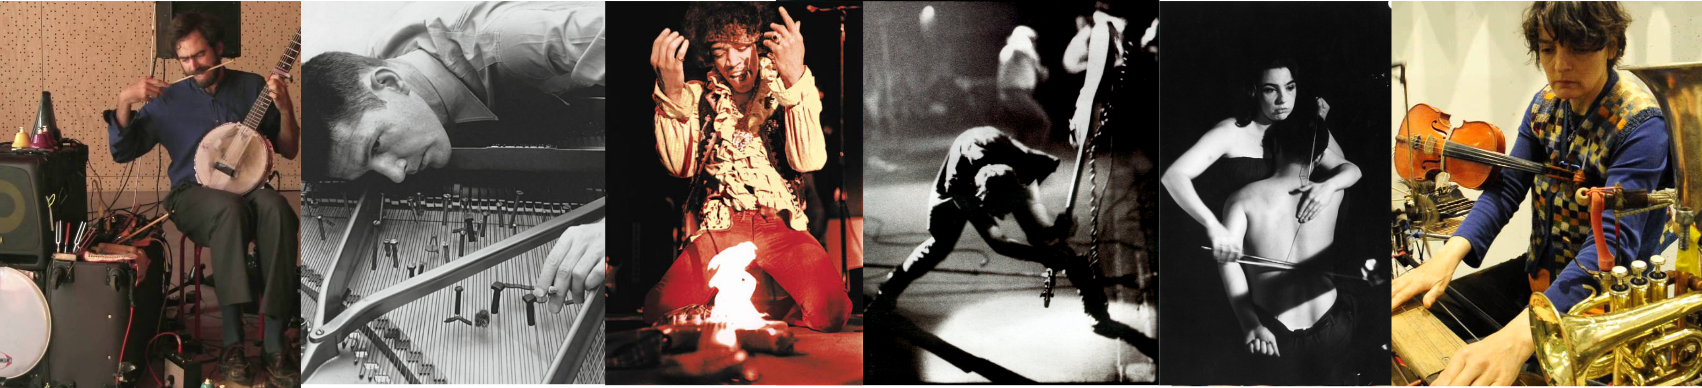
\includegraphics[width=\textwidth]{gfx/03_gesture/instrumentabusers.png}
	\caption[Les instrument ne sont pas des interfaces utilisateur]{Les instrument ne sont pas des interfaces utilisateur. De gauche à droite : Thomas Bonvallet, John Cage, Jimi Hendrix, Paul Simonon, Charlotte Moorman, Sarah Kenchington}
	\label{fig:gesture:abusers}
\end{figure}
%---- Figure : Einarsson sculpture ---------
\noindent Or dans une performance musicale vivante, cette situation n'existe pas. Le musicien ne saurait être défini comme ``l'utilisateur de son instrument''(figure \ref{fig:gesture:abusers}), pas plus que son instrument comme une ``interface utilisateur''. Les musiciens cherchent bien souvent à produire quelque chose à la limite des possiblités de leur instrument\footnote{cf. interview de Nicolas Bernier désignant ``l'infini des possibles'' comme principale motivation l'ayant amené à utiliser les instruments électro-acoustiques.}. Que cela soit le contre fa de la Reine de la Nuit, les partitions impossibles de Brian Ferneyhough, les pianos préparé de John Cage, le scratch sur les platines vinyle ou les mises en larsen de table de mixage de la scène Onkyokei, les exemples abondent dans l'histoire de la musique qui font preuve d'une démarche allant dans l'outrepassement des possibilités instrumentales lors du jeu musical. Dans une conversation durant la dernière conférence NIME, Paul Stapleton utilisait ironiquement le terme \textit{interface abusers} pour souligner l'erreur du terme \textit{interface users}. \footnote{Un exemple significatif de cette différence entre usage et abus de l'instrument est la réduction de la hauteur dans le format MIDI à un paramètres entier borné entre 0 et 127 pour contrôler la hauteur—ce qui excède déjà la tessiture du piano à 88 touches. Les fréquences audibles excèdent largement cette tessiture, et certains genres de musiques électroniques, comme l'\gls{IDM} ou le \gls{glitch}, ont précisément fait de l'utilisation de fréquences suraigues ou infra-basses une de leurs composantes esthétiques.}


nément admis comme des qualités requises pour l'interaction instrumentale.
Le problème de toute catégorisation est qu'elle peine à rendre compte des chevauchements et intersection entre ses catégories. Nommément, les gestes subversifs peuvent être de nature excitatoire tout en jouant sur le \textit{pré-geste} (sound-facilitating) pour lui faire dire le contraire.

D'autres descriptions du geste telles que celles employées dans l'apprentissage traditionnel du Guqin, consistant à décrire le geste par l'image de la position de main, associée à l'image d'un animal et d'un texte poétique décrivant l'esprit du mouvement, par exemple ``A la manière d'une grue qui danse parce qu'elle est effrayée par une brise.''

D'un certain point de vue, on pourrait dire que cela n'a pas de sens de vouoir jouer d'un \gls{DMI} de manière \textit{transparente} dans la mesure où les gestes sont subvertis à la source même de l'interaction. C'est en quelque sort un mésusage de l'informatique qui consiste à l'utiliser comme si les \glspl{DMI} étaient des synthés analogiques (dans lesquels une certaine continuité énergétique subsiste entre les capteurs et le son).


Il a été souvent déclaré comme critère de design des DMIs qu'ils se devaient d'être très réactifs. Cependant, si cette caractéristique est éminnement présente dans les instruments acoustiques où l'énergie gestuelle est transformée et traduite de manière continue et instantanée dans le son, ce n'est pas le cas des instruments numériques. Mais au lieu de voir cela comme un défaut, considérons cette caractéristique qui en découle : le fait de ne pas constamment devoir agir pour entretenir un son sur un \gls{DMI} libère l'esprit pour s'occuper de gérer des formes à plus long terme. Le live-coding (ou plutôt, les musiques séquencées, de manière générale) est quasi uniquement dans ce mode d'interaction ou les actions sur le clavier n'ont de conséquence sur le son qu'un fois les commandes validées et que l'état du séquenceur permet la prise en considération de la modification du pattern.

%-------------------------------------------
\subsection{Se départir du modèle acoustique}

Les études du geste musical qui ont amenée à la classification ci-dessus ont essentiellement été menée sur des instruments acoustiques, pour lesquels la relation entre le geste et le son est généralement causale, immédiate, et caractérisée, dans la plupart des cas, par un transfert énergétique proportionnel.
Par ailleurs et jusqu'à récemment, la tradition musicale de l'IRCAM de composition pour instruments acoustiques classiques et la relégation quasi-systématique de la partie électronique des compositions\footnote{synchronisée—et non jouée, par des \gls{RIM} et non des musiciens} dans l'ombre de l'arrière-scène n'a guère favorisé la considération des interfaces électroniques et des nouveaux gestes qui leur étaient propres en tant qu'instrument de performance musicale à part entière.

%-------------------------------------------
\subsubsection{continuum énergétique}

Claude Cadoz accorde une grande importance à la question du continuum énergétique, et considère que l'interaction physique ``par contact'' avec l'instrument est une condition nécessaire pour pouvoir qualifier un geste d'instrumental. Non seulement le continuum énergétique doit être assuré pour que l'énergie gestuelle soit retrouvée dans le son produit, mais l'interface doit opposer un retour d'effort dynamique pour assurer la bi-directionnalité du canal gestuel.

\iquote{Nous touchons ici un point crucial, car c’est précisément cette unidirectionalité qui rend ces systèmes inaptes à assurer la fonction ergotique du canal gestuel. La présence simultanée de capteurs et d’effecteurs dans le dispositif d’interface gestuelle est en effet une condition nécessaire à cette fonction.}\cite{cadoz_musique_1999}

La description des fonctions du geste instrumental pour les instruments acoustique l'amène à poser la fonction ergotique (celle qui fournit l'énergie) comme base nécessaire pour le design des interfaces musicales. Cette condition requise de l'instrumentalité a éminemment poussé l'équipe de l'\gls{ACROE} dans des développements singuliers et intéressants à plus d'un titre. 

On ne saurait pour autant, en considérant le paysage des pratiques musicales actuelles avec des \glspl{DMI}, accepter un tel critère comme une condition de leur existence. Par ailleurs, il semble paradoxal de vouloir préserver la continuité énergétique lors de l'usage d'un dispositif numérique qui, par nature, rompt cette continuité\footnote{Ajourdh'hui encore, malgré de récents développements notamment sur la base de système Hamiltonien à ports (cf Hélie), le bilan énergétique n'est pas préservé lors de la quantification et de l'échantillonage de signaux analogiques. TODO : développer un peu ou supprimer}. 



Si l'introduction de l'électricité a entrainé un découplage énergétique, l'introduction de l'informatique a opéré un découplage de la causalité. Le son numérisé n'est pas directement le courant électrique qui va \textit{in fine} faire bouger la membre d'un haut-parler, c'est une image, une représentation de ce signal. Il en va de même pour les gestes numérisés. Il n'y a plus de continuité (même électrique!) dans l'interaction énergétique, mais une succession d'opérations discrètes qui simule une continuité. 


\subsubsection{La latence du temps-réel}

Remarquons à ce propos que si l'on a beaucoup utilisé le terme de ``temps-réel''\footnote{Comme par exemple dans la dénomination de l'équipe de l'IRCAM dévolue au développement d'objets pour le traitement du son en ``temps-réel'', nommée successivement ``Equipe Application Temps-Réel'', puis ``Interactions Musicale Temps-Réel'', afin de finalement abandonner ce terme de temps-réel pour s'appeler ``Sound Music Movement Interaction''.} lorsque sont arrivés les premiers synthétiseurs permettant un calcul du son à une fréquence plus rapide que celle de son échantillonage, il ne faut pas oublier que l'ordinateur n'a pas tant introduit le ``temps-réel'' que le ``temps différé''.
Mais il a fallu tant d'effort pour arriver à réduire cette différance en deça des seuils perceptible, et produire les premiers instruments numériques s'approchant de l'immédiateté naturelle des instruments acoustiques, qu'elle a pour ainsi dire éclipsé la disposition des machines à produire du temps différé dans une perspective instrumentale.


Large développement d'outils pour la gestion "offline" de la musique (déplacement, copié/collé,etc) et de l'ergonomie de ces outils.
Hybridation des instruments entre du controle instrumental direct ("traditionnel") et des techniques issues de la production musicale offline.


accorde à la musique le droit de \iquote{tromper l'oreille} (et la vue).

\subsubsection{lisibilité, répétabilité, fiabilité, fidélité}

Pendant longtemps (TODO : combien?), les instrumentistes utilisant des \glspl{DMI} ont été cachés derrière des machines, à la position souvent occupé par l'ingénieur du son, ne laissant rien voir ou si peu de ce qu'ils faisaient vraiment. Pire, ils se trouvaient suspectés, quand ils étaient sur scène, de faire semblant de jouer. \cite{cascone_aesthetics_2000}


Expliquer en quoi le découplage énergétique, qui a amené à "un sens de la discontinuité avec la tradition, aliénation et manque de compréhension par le public en ce qui concerne ce que l'instrumentiste ou l'instrument fait en réalité". (T Magnusson, in \cite{magnusson_sonic_2019} pp. 61) a amené à une contre-réaction faisant passer la lisibilité 


\subsubsection{transparence}

Louange de la transparence : \cite{fels_mapping_2002} 
\iquote{We consider transparency as a predictor for expressivity. (...) We identify transparency as a quality of a mapping.}

\iquote{Another basic need is that the software provide correspondences between input data and output sound that are sufficiently intuitive for both performer and audience.}\cite{dobrian_e_2006}



\subsubsection{fidélité}

La notion de ``fidélité'' est également vantée dans les dispositifs technologiques comme un gage de qualité. Fernando Iazzetta \cite{iazzetta_meaning_2000} analyse la manière dont la notion de fidélité dans l'industrie musicale, orginalement utilisée pour désigner la capacité d'un enregistrement à reproduire les qualités sonores de la performance originale, a progressivement vers une notion de fidélité non plus basée sur le son original lui-même, mais établie en fonction de la technologie d'enregistrement disponible. La situation actuelle (de la musique pop en particulier) dans laquelle l'écoute, voire la production en studio, d'un enregistrement précède l'écoute de la performance elle-même amène ainsi de nombreux musiciens à une situation paradoxale, consistant à chercher à reproduire dans leurs performances live les mêmes qualités sonores que celles de leurs disques.


de la relation geste/son comme un critère pertinent de design instrumental.


\subsubsection{incompréhension}
Parmi les aspects qui reviennent le plus souvent pour décrire la relation qui s'établit dans une performance entre le musicien et l'auditeur, il est celui de la ``compréhension'' par le public de ce que le musicien fait sur scène (e.g. \cite{schloss_using_2003}, \cite{fels_mapping_2002}) et l'incapacité à faire soi-même cette performance.

Si la cause parait consensuelle, je dois avouer que j'ai ressenti l'exact inverse de trop nombreuses fois pour adhérer pleinement à cette thèse. Bien souvent, des performances musicales tout à fait obscures et incompréhensibles, dépourvue de virtosité gestuelle démonstrative, m'ont davantage intéressées que les gesticulations visibles et prévisibles d'une performance, même virtuose. Je n'irai pas jusqu'à prétendre qu'il y a là une tendance universelle, mais j'imagine ne pas être le seul à avoir ce goût là —surtout dans la recherche— de m'intéresser à des musiques que je ne comprends pas.



\iquote{Si ça se trouve, cette notion que dans quelques années, ``tout sera possible avec la technologie'' fera que cela sera compliqué de créer un mystère entier et profond, parce que les gens du coup diront ``oui, j'en ai entendu parler, maintenant on peut faire ça''.
 J'ai un ami (...) qui a fait voler un espèce de morceau de tulle au dessus des gens avec des principes mécaniques, et beaucoup de gens disaient ``ah oui, c'était incroyable mais je pense que c'était un drône'', alors que pas du tout. Mais je me suis dit, c'est vrai que d'ici quelques années, un objet qui vole tout seul en silence dans l'espace, n'aura plus le même pouvoir de mystère qu'il y a quelques années.} Yann Frish dans \url{https://www.youtube.com/watch?v=5BqHXbQC36M}





%%%%%%%%%%%%%%%%%%%%%%%%%%%%%%%%%%%%%%%%%%%%%%%%%%%%%%%%%%%%%%%%%%%
%%%%%%%%%%%%%%%%%%%%%%%%%%%%%%%%%%%%%%%%%%%%%%%%%%%%%%%%%%%%%%%%%%%%
\section{Geste programmé, geste re-sonné}
\label{sec:gesture:instrumental_to_musical}
%-------------------------------------------
\subsection{L'outil comme externalisation de la mémoire}
\label{sec:gesture:instrumental_to_musical:externalisation}

\noindent Dans son essai ``Le geste et la parole'' paru en 1964 \cite{leroi-gourhan_geste_1964}, le paléo-anthropologue André Leroi-Gourhan met notamment en lumière la manière dont l'invention et l'utilisation d'outils techniques contribuent à l'évolution de l'humain, par un processus d'externalisation progressive des processus opératoires dans les outils :\\
\iquote{Au cours de l’évolution humaine, la main enrichit ses modes d’action dans le processus opératoire. L’action manipulatrice des Primates, dans laquelle geste et outil se confondent, est suivie avec les premiers Anthropiens par celle de la main en motricité directe où l’outil manuel est devenu séparable du geste moteur. A l’étape suivante, franchie peut-être avant le Néolithique, les machines manuelles annexent le geste et la main en motricité directe n’apporte que son impulsion motrice. Au cours des temps historiques la force motrice elle-même quitte le bras humain, la main déclenche le processus moteur dans les machines animales ou les machines automotrices comme les moulins. Enfin au dernier stade, la main déclenche un processus programmé dans les machines automatiques qui non seulement extériorisent l’outil, le geste et la motricité, mais empiètent sur la mémoire et le comportement machinal.}\cite{leroi-gourhan_geste_1964} pp 41-42\\
\indent Il note ainsi que l’externalisation des facultés de l'humain s’est étendue à tous ses organes, jusqu'aux fonctions cérébrales de la mémoire, et prédit les opérations de computabilité rendue possible par le numérique :
\iquote{Les fichiers à perforations sont des machines à rassembler des souvenirs, elles agissent comme une mémoire cérébrale de capacité indéfinie, susceptible, au-delà des moyens de la mémoire cérébrale humaine, de mettre chaque souvenir en corrélation avec tous les autres.} \cite{leroi-gourhan_geste_1964} p 74.

cf. Magnusson outil épistémique

%-------------------------------------------
\subsection{Le geste programmé}
\label{sec:gesture:instrumental_to_musical:geste_programme}

\noindent Le geste peut être réalisé explicitement par un instrumentiste humain ou bien produit de manière automatisée par la machine; on pourra alors parler de gestes programmés. Leur définition peut être ``extensive'', par exemple sous la forme d'enregistrements (samples, courbes d'automation, etc. (cf. Figure \ref{fig:gesture:automation})) ou ``intensive'', c'est-à-dire définie par une règle qui permet à un processus de la générer) \footnote{Sur les notions de notation ``intensive'' et ``extensive'', voir Giavitto \cite{giavitto_du_2014}}. Si toutefois la définition du geste implique que le mouvement soit associé à une intention, on ne peut prêter une intention à la machine qu'à travers la ``programmation'' de ce mouvement machinique par le compositeur/luthier numérique.
%------------------ Figure : geste programmé ---------------------
\begin{figure}[!htbp]
	\captionsetup{format=plain}%
	\centering
	\begin{minipage}[t]{0.48\textwidth}
		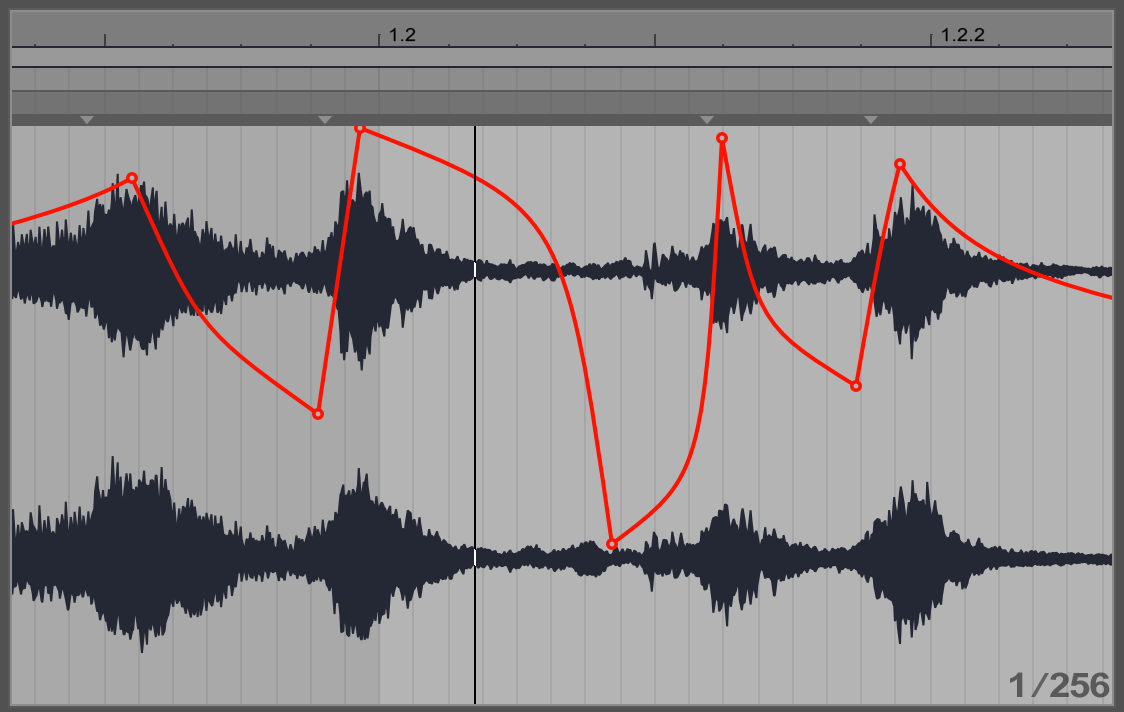
\includegraphics[width=\linewidth]{gfx/03_gesture/AbletonLiveAutomation_72dpi.png}
		\caption{Une courbe d'automation dans le logiciel Ableton Live}
		\label{fig:gesture:automation}
	\end{minipage}
	\hspace{.02\linewidth}
	\begin{minipage}[t]{0.48\textwidth}
	  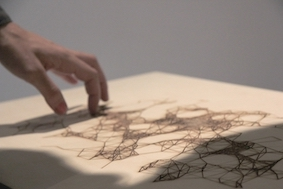
\includegraphics[width=\linewidth]{gfx/03_gesture/EnriqueThomas-TangibleScore_72dpi.jpg}
		\caption{Partition tangible d'Enrique Tomás}
		\label{fig:gesture:tangible_score}
	\end{minipage}
\end{figure}
%------------------ Figure : geste programmé ---------------------
\indent Stiegler développe le concept de ``gramme'' comme \iquote{corps organisé de signes et de symboles} et emprunte à Sylvain Auroux \cite{auroux_revolution_1994} le concept de ``grammatisation'' comme \iquote{le processus par lequel le continuum temporel des comportements humains est transformé en un spatial discret, qui permet de les intégrer dans les outils}. Ainsi en est-il de l'informatique, qui dissocie en symboles et en catégories discrètes ce qui est continu et intégré dans le geste, comme dans le son. Pour Stiegler, les objets sont des enregistrements\footnote{Stiegler utilise les termes de ``rétentions tertiaires'' pour décrire cette inscription de la mémoire dans les objets, afin de la mettre en perspective des ``rétentions primaires'' que sont la conscience du flux temporel et les ``rétentions secondaires'' que sont les souvenirs qui constitue l'expérience d'un individu.}, dans laquelle la mémoire de ce que nous faisons et de ce que nous connaissons est déposée sous la forme d'une mémoire technique. L'instrument de musique contient ainsi l'enregistrement de la théorie musicale qui lui est propre (son organisation des hauteurs, sa signature timbrale, son ergonomie, etc.) et que le luthier lui imprime. De même, la partition est un enregistrement de la pensée et du travail du compositeur, une trace de ses ``gestes sédimentés'' comme le dit Jean-Paul Olive dans \cite{olive_expression_2013}.

Une autre notion se rapprochant de l'idée de geste programmé est celle de ``diagramme'', proposée par Gilles Deleuze dans son étude sur la peinture de Francis Bacon \cite{deleuze_francis_1981}.
\iquote{Un diagramme peut immobiliser un geste, le mettre au repos, bien avant qu’il ne se blottisse dans un signe, et c’est pourquoi les géomètres ou les cosmologistes contemporains aiment les diagrammes et leurs pouvoirs d’évocation préemptoire..} Gilles Châtelet, cité par Mazzola, Topos of music III, p. 68


On voit dans ce concept de ``geste programmé'', la rencontre du travail du luthier et du compositeur qui fait écho à la frontière devenue floue entre ces deux aspect de la création musicale: l'instrument est ``composé'' \cite{schnell_introducing_2002}, la partition est ``instrumentalisée''\footnote{Voir à ce sujet le travail explicite de Enrique Tomás sur les ``partitions tangibles'' \cite{tomas_tangible_2014}}.

\iquote{In the case of “programmable instruments” and live control of compositional computer music algorithms, the distinction between compositional expression and performative expression may be blurred somewhat; the performer may be shaping primary characteristics of the composed/improvised musical materials themselves.}\cite{dobrian_e_2006}


\iquote{Quant à la duction de l'instrumentiste, elle vient retemporaliser ce qui ne peut être que spatial : le travail de la composition, ce n'est que spatial, c'est du temps spatialisé, et en cela, essentiellement en défaut d'être. C'est du virtuel pur. C'est du temps discrétisé et détemporalisé dans cette mesure. Discrétisé, il devient manipulable dans sa détemporalisation temporaire telle que la pratique le com­positeur, mais il n'est que virtuel. Il ne peut devenir actuel qu'avec l'interprète, qui doit le re-temporaliser.} B. Stiegler dans \cite{stiegler_circuit_2004}

Cependant, il ne faudrait pas prendre ces ``gestes programmé'' pour de simples enregistrements à repoduire tels quels. La perspective de performance musicale à partir de ces gestes programmé suppose un ``jeu'' avec le geste enregistré, sinon ce ne serait pas un musicien mais, justement, un utilisateur qui démarre, par exemple, la lecture d'un enregistrement audio. La performance musicale consiste justement à faire entendre ce qui n'est pas calculable comme le dit Stiegler \cite{stiegler_circuit_2004}:
 
 \iquote{Un musicien, c'est quelqu'un qui d'abord entend, c'est-à-dire qu'il est primordialement affecté par l'oreille, une oreille qui a cependant des yeux et des mains, et un corps qui les relie. Il ne se contente pas de calculer. Il peut calculer, il doit même calculer, mais s'il le fait, c'est pour donner à entendre ce qu'il a lui-même entendu comme l'incalculable même.}

 Ces gestes programmés ne sont donc pas de simple enregistrements linéaire, mais des modèles complexes et dynamiques qui invitent à des gestes de re-sonnance (voir section suivante) et auxquels la notion de ``modèle intermédiaire dynamique'' (cf. \ref{sec:algorithms:MID}) fait écho.

 Cette part incalculable dont parle Stiegler fait écho à la propension du geste à dépasser ses propres limites, non pas seulement sur le plan physique mais également sur le plan cognitif. (cf. example des musiques de Steve Reich, d'abord créées avec l'aide de machine, puis de manière humaine => piano phase solo)

\textbf{Extra notes}\\

Geste composé (écrit, enregistré, extrait d'analyse, ...) sous forme intensive ou extensive et produit par les machines.\\
Mouvement des machines (cf. Patrick Saint Denis machines mobiles)\\
Mouvement dans l'image (cf. Serge de Laubier musique visuelle => festival, \iquote{amplifier l'écoute par l'image})\\
\iquote{Musique, Incarnation, physique, informatique, voilà quatre fusions de l'alliage dur-doux. (...) Nous nous étonnons devant ces quatre miracles, ces quatre fusions, parce que nous manquons d'une philosophie du mélange} Michel Serres, Musique


%-------------------------------------------
\subsection{Le geste de re-sonance}

Nous avons vu que le geste musical peut se retrouver incorporé dans le corps de l'instrument sous forme de geste programmé. Ce geste programmé appelle à la mise en mouvement temporelle par le musicien.
Dans le cas de l'instrument acoustique, l'instrument pris isolément est un système passif dont la résonance est purement acoustique : les modes de vibrations propres des corps résonant de l'instruments répondent aux gestes d'excitation et il est possible de modéliser cette résonance acoustique en mesurant la réponse impulsionelle de l'instrument.

Cependant, l'instrument ne joue pas seul et le couple instrument/instrumentiste n'est plus un système passif puisque l'instrumentiste apporte une énergie et vient moduler le son on modifiant les modes acoustiques qui conditionne la durée de vie (ou d'extinction, selon la persepctive adoptée) du son.

Dans le cas de l'instrument numérique, le système est actif et le geste de re-sonance est un geste de manipulation interactive du geste\/son programmé.
Il s'agit à la fois de faire sonner ce qui est latent dans le son, mais également de trouver la relation spatio-temporelle d'interaction qui va permettre à l'instrument de sonner comme on le souhaite et de ``jouer'' avec le geste programmé.

Le geste de ré-sonance, ou de ré-animation \footnote{La thèse de Norbert Schnell \cite{schnell_playing_2013} propose une étude théorique et pratique de scénarios de ré-animation pour le cas de sons enregistrés.}, implique à la fois la chorégraphie du geste et la spectromorphologie du son\footnote{sur la spectromorphologie du son, voir Christopher Small}, dans une relation de correspondance. Cette relation est doublement dynamique, dans la mesure où le geste et le son ont leur propre mouvement interne d'une part, et dans la mesure où ils s'influencent l'un l'autre. Ainsi, la relation de ``résonance du geste'' se construit sur le plan [fonctionnel du geste] instrumental en même temps que sur le plan [métaphorique du geste] musical.

Un exemple significatif est l'interprétation de ``Hangsimogato N°2'' de György Kurtág Jr\footnote{Vidéo disponible sur \url{https://www.youtube.com/watch?v=MJ8Z5skovLw}}. Dans cette pièce, le développement musical se fait par avancement sur une partition pré-programmé par l'intermédiaire d'un capteur Infra-Rouge (D-Beam). Le capteur lui-même n'est pas sensible à l'orientation de la main ou à quelle main (gauche ou droite) vient couper le rayon, mais György Kurtág Jr développe tout un vocabulaire gestuel qui établit des relations de correspondance avec le son. Ces relations de correspondance peut s'appuyer sur une similarité de morphologie énergétique, mais dans certains cas (e.g. geste de présentation des mains ouvertes vers le ciel, replis des bras en croix) elle sont purement métaphoriques et poétiques.

\todo{rajouter un screenshot de la vidéo de Gyorgy}

Parler de l'IA, notamment l'écrite de la relation geste/son à partir de mécanismes d'apprentissage machine et de corrélation, tel que dans Wekinator

\subsubsection{ADSR gestuel}


\subsubsection{geste de production du son et geste d'extinction du son}

Dans les instruments acoustiques, le seul paramètre sonore généré par l'instrument seul est sa résonance.
Si dans les instruments acoustiques, l'extinction du son est une donnée inhérente à leur propriétés physiques (les instruments acoustiques étant des systèmes passifs dans lesquels le son décroit inexorablement et s'éteint s'il n'est pas entretenu), les instruments électriques (dont les instruments électroniques et les \glspl{DMI}) nécessitent que le son soit explicitement éteint, que cela soit assuré de manière automatisée, via la programmation de l'instrument, ou par un geste venant commander cette extinction.

Le geste de répétition, qui est explicite chez l'instrumentiste classique, s'il souhaite refaire entendre un passage, et est automatisé dans le concept de boucle.

Geste de spatialisation (cf. Bertrand Merlier, Pierre Couprie), de projection. (qui n'est pas simplement une ``modulation'')

Toutes les composantes du son, de la musique, et de la scénographie sont sujettes à l'invention de gestes, selon ce que le musicien décidera comme d'importance pour sa musique.



%%%%%%%%%%%%%%%%%%%%%%%%%%%%%%%%%%
\section{Subversion sonore, subversion gestuelle}
\label{sec:gesture:subversion}
%------------------ Figure : geste lisible ou subversif ---------------------
\begin{figure}[!htbp]
	\captionsetup{format=plain}%
	\centering
	\begin{minipage}[t]{0.48\textwidth}
		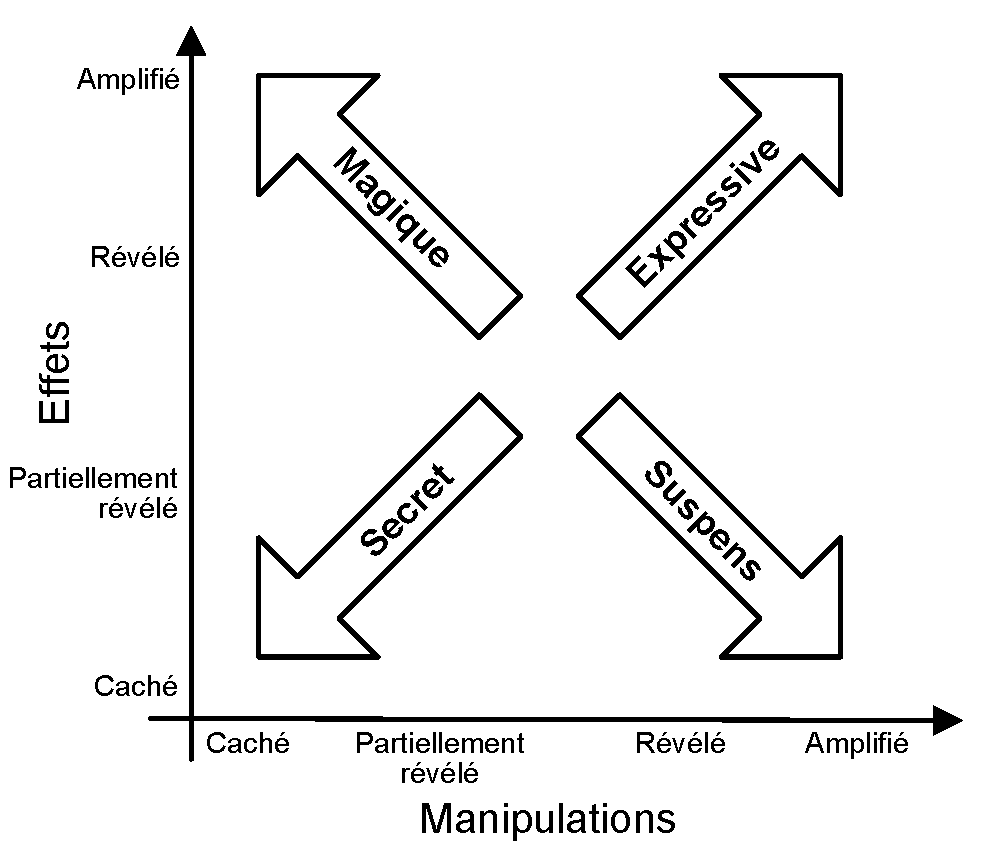
\includegraphics[width=\linewidth]{gfx/03_gesture/ManipulationVsEffect2.pdf}
		\caption{Visibilité de la manipulation et de l'effects (``Strategies for designing spectator interfaces.'') dans \cite{reeves_designing_2005, benford_performing_2010}}
		\label{fig:gesture:Benford}
	\end{minipage}
	\hspace{.02\linewidth}
	\begin{minipage}[t]{0.48\textwidth}
	  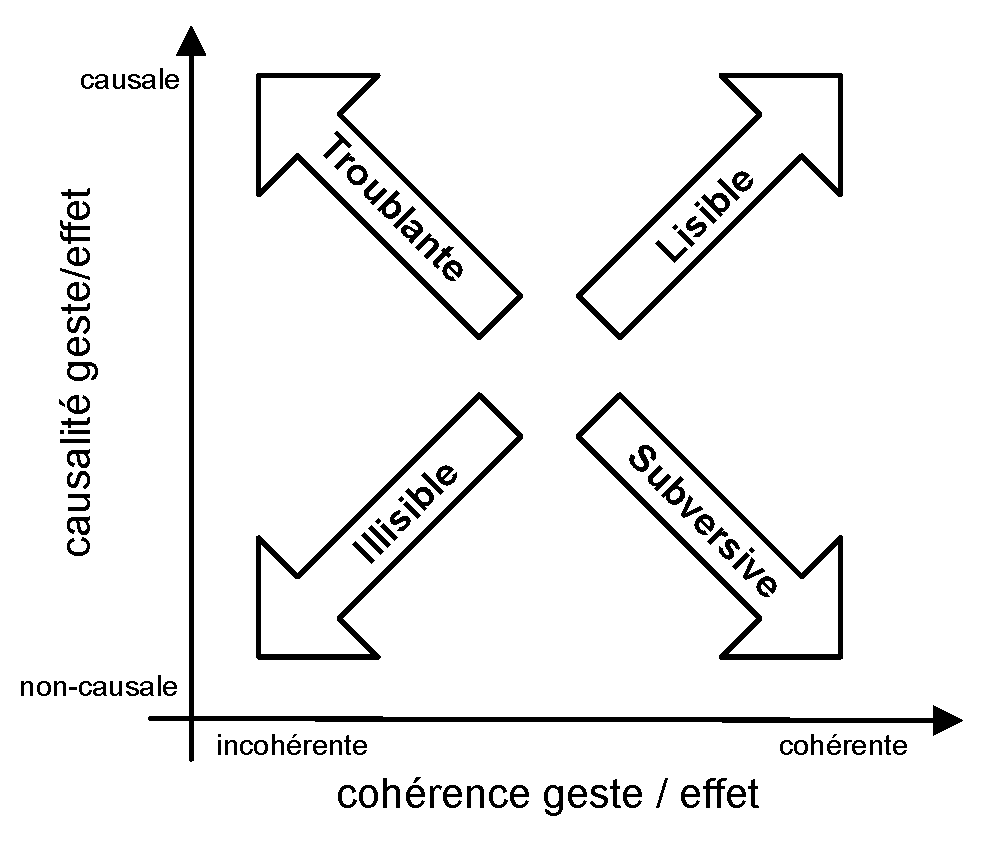
\includegraphics[width=\linewidth]{gfx/03_gesture/CoherenceVsCausalite2.pdf}
		\caption{Lisibilité et subversivité de la relation geste/effet}
		\label{fig:gesture:lisibility_subversion}
	\end{minipage}
\end{figure}


Perception d'erreur du point de vue du spectateur \cite{fyans_ecological_2012}

Dans la figure de Benford manque la possibilité que la visibilité ne soit pas causale de l'effet.

lisible : on voit et on entend une personne parler
illisible : on voit une personne parler et on entend une autre voix
subversive : le playback
troublante (dissonance cognitive entre vue et ouïe): le ventriloque

\subsection{Définition} 

Le terme ``subversion'' (du latin \textit{subvertere} : renverser, bouleverser) désigne ``l'action visant à saper les valeurs et les institutions établies'' (dictionnaire Larousse). Les moyens employés par la subversion consiste à diffuser un message contraire à un l'ordre établi, dans le but d'affaiblir celui-ci.

Dans le cas de la musique, si la notion de subversion peut prendre une dimension culturelle ou politique dans certains courants musicaux, c'est ici dans le cadre de la perception que j'emploie ce terme.

La subversion peut intervenir à différents niveaux. Au niveau de la composition, l'écriture musicale permet des modulations qui déjouent les attentes de l'auditeur. (e.g. Pink Floyd, breathe transition). Elle peut également se situer au niveau du jeu, en usant de procédés comme des gestes qui contredisent ce qu'on entend et vont l'amplifier. Gyorgy Kurtag Jr. geste violent pour jouer une nuance pianissimo.

Exemples comparés de Applebaum Aphasia et Vincent Carinola/Jean Geoffroy "Virtual Rhizome".
BBC Classic Album: "Pink Floyd - The Dark Side of the Moon"

Dissonance cognitive.

Synchrèse de Michel Chion.

Parler du playback, du air-guitar, de la synchrèse.

Nattiez, Music and discourse p44 : certain pianistes ont l'impression de donner de la ``profondeur'' à un accord en permettant aux doigts de glisser vers l'intérieur du piano après avoir enfoncé les touches. (...) inversement, Braendel : le son de notes soutenues sur le piano peut être modifié... à l'aide de certains mouvements qui rendent la \textit{conception du cantabile} du pianiste visible pour le public. (Delalande, ``vers une psycho-musicologie'' in L'enfant du sonore au musical):166, (Brendel, A. 1976. Musical Thoughts and Afterthoughts. Princeton: Princeton University Press. p.31)

Bien que ces catégorisations du gestes décrivent adéquatement différents aspects du geste instrumental sur des instruments acoustiques, il semble que le geste musical intègre une aspect subversif souvent négligé.

En particulier, dans le cas des \glspl{DMI}, la relation entre le geste et le son est totalement sujette au design de ce que l'on nomme communément le \gls{mapping} et la part de subversion devient partie intégrante du design de ce mapping. 


Il semble dès lors que l'on peut envisager d'autres types de relation entre le geste et le son, afin de tenter de décrire les différents rapports qu'ils entretiennent selon les situations.

Risset fait remarquer l'importance de l'histoire du son d'origine mécanique dans la perception des sons \cite{risset_son_1992}: 

\begin{quotation}
II semble à première vue que l'acoustique numérique puisse s'affranchir de la mécanique. Cependant notre ouïe a évolué dans un environnements d'objets vibrants: aussi la prise en considération des contraintes et des particularités des vibrations mécaniques est-elle importante pour comprendre les idiosyncrasies de la perception auditive et pour en tirer parti.

Les limites de l'acoustique numérique dépendent des capacités différentielles de perception davantage que des contraintes mécaniques. Pourtant, notre perception auditive est orientée par un monde de sons produits mécaniquement, et la mécanique ne doit pas être écartée de façon cavalière, comme l'ont suggéré les travaux de Gibson et Cadoz : les spécificités des vibrations mécaniques mettent en lumière l'organisation perceptuelle dans le processus auditif


\footnote{The limitations of digital acoustics depend upon the differential capacities of perception rather than upon the constraints of mechanics. Yet our auditory perception is geared to a world of mechanically-produced sounds, and mechanics should not be given a cavalier dismissal, as the work of Gibson and Cadoz has suggested : the specifics of mechanical vibrations shed light on the the perceptual organization in the hearing process.} TODO : traduire l'anglais, plus riche.
\end{quotation}


\textbf{Proposition}
\vspace{-1em}
\begin{itemize}[noitemsep]
\item readable gesture to sound relations
\item confusing gesture to sound relations
\end{itemize}

\vspace{-1em}
\begin{itemize}[noitemsep]
\item Gestes emphatique = en phase avec le mouvement interne du son
\item Geste apophatiques = en opposition de phase avec le son
\item Geste unrelated
\end{itemize}

%---- Figure : Einarsson sculpture ---------
\begin{figure}[!htbp]
	\captionsetup{format=plain}%
	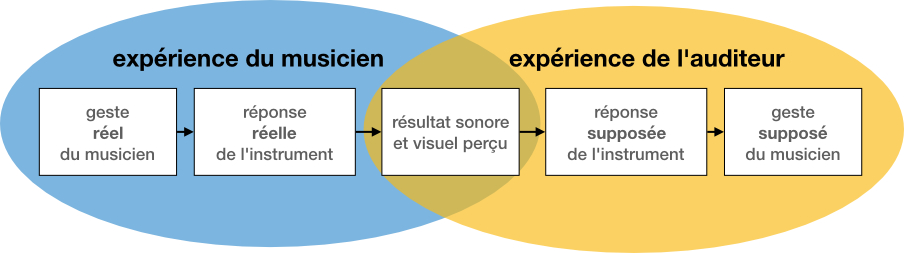
\includegraphics[width=\textwidth]{gfx/03_gesture/gesteReelGesteSuppose.jpg}
	\caption{Geste produit, geste perçu, fonctionnement réel et supposé de l'instrument}
	\label{fig:gesture:RealVsSupposed}
\end{figure}


%-------------------------------------------
\subsection{Sons paradoxaux, gestes paradoxaux}
Risset, Kurtag Jr., Kurtag Père

De la même manière que l'écriture musicale sur papier a permi de développer des processus de compositions difficilement pensables sans ce support visuel \footnote{tels que la rétrogradation ou la fugue}, les ordinateurs ont permi de créer des formes sonores qu'il aurait été impossible de concevoir sans cet outil computationnel, tels que les sons paradoxaux de Risset et Shepard \footnote{qu'il n'est toutefois pas impossible de reproduire sans recourir à l'ordinateur, telle démontrée que cette interprétation des glissandi de Risset à la voix par Victoria Hart \url{https://vimeo.com/147403169}}

Si les catégories gestuelles décrites par Cadoz et Wanderley se prêtent à la description des gestes sur un instrument acoustique, elle semble inadaptées ou insuffisantes pour décrire la fonction du geste dans une perspective musicale, en prenant en compte à la fois l'aspect sonore mais également l'aspect scénographique de la performance musicale.

\vspace{-1em}
\begin{itemize}[noitemsep]
\item \textbf{gestes de feintes} : déception de l'attente, mais visible après coup. E.g. dans le football, faire semblant d'aller à droite et envoyer le ballon à gauche, en musique: ommettre le temps fort d'un rythme bien établi, etc. La mécanique du geste est entièrement visible mais a été confuse par un changement innatendu.
\item \textbf{geste magique} : La mécanique du geste reste invisible et la logique causale entre le geste et son résultat reste inexplicable, et sujette à spéculation imaginaires.
\end{itemize}


%---- Figure : Triggering modes ---------
\begin{figure}[!htbp]
	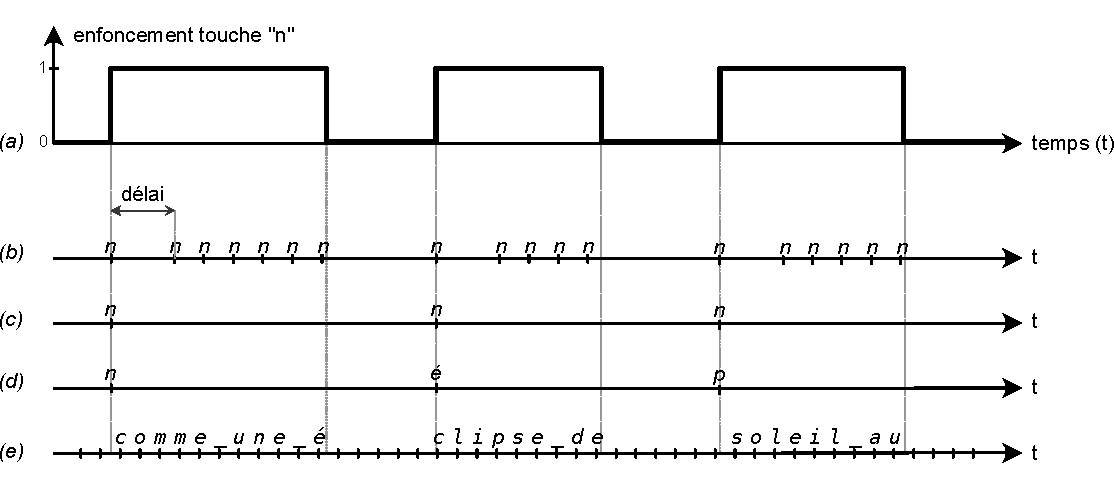
\includegraphics[width=\textwidth]{gfx/03_gesture/key_modes.pdf}
	\caption{Différents modes de déclenchement: (a) enfoncement de la touche ``n''; (b) comportement habituel d'un clavier (e.g. dans un traitement de texte) (c) suppression de la répétition (d) utilisation d'un réservoir (e) phrases séquencées rythmiquement}
	\label{fig:gesture:triggering_modes}
\end{figure}


%-------------------------------------------
\subsection{Continuités artificielles}

\vspace{-1em}
\begin{itemize}[noitemsep]
\item Contrepoint : relier la mélodie à l'harmonie 
\item Bach et le tempérament = relier les différents modes, via la modulation.
\item les doigtés alternatifs, sur le plan gestuel, permettent de sacrifier la justesse de la note, pour établir une continuité gestuelle fluide
\item La musique sérielle : relier la gamme tempérée au spectre en ordonnant 
\item Stravinsky, Russolo : relier l’harmonie et le bruit 
\item jouer un pattern connu ("qu'on a dans les doigts") tout en substituant les notes permet de jouer de manière fluide une mélodie inhabituelle. => numérique
\item Cage, Murray Schaeffer : relier le déterminisme et le hasard, la musique et l’environnement 
\end{itemize}

(morpho-dynamisme)
Mettre capture d'image du MID qui passe d'une structure rotative à un Verlet.

Comment la continuité s'établit ?

=> voir Théories de la composition musicale au \siecle{20}~siècle
Conjointement à ces explorations compositionnelles se sont développées des techniques et des technologies permettant d’appréhender ces nouveaux espaces. Que cela soit des procédés d’écriture ou des instruments reflétant ces méthodes et modèles.

\subsection{L'importance du format de données}
La possibilité d'établir des continuités entre des espaces gestuels et sonores dépend en partie de la possibilité d'exprimer cette espace dans le format de données adéquat. Par exemple, exprimer une grande polyphonie dont le nombre d'élément est fixe sera probablement plus facilement exprimable à l'aide de matrices, alors que des événements distincts sera plus aisément exprimés sous formes de messages indépendant. De la même manière, des événements déclencheurs peuvent être facilement exprimés sous la forme de messages asynchrones tels que des messages MIDI, mais le flux de ces événements devient très rapide et que leur rythme importe, il sera peut-être plus efficace de les délencher à l'aide d'un signal synchrone tel qu'un signal audio. Cf. Stockhausen Kontakte.

%%%%%%%%%%%%%%%%%%%%%%%%%%%%%%%%%%%%%%%%%

\section{Résonance entre le geste re-sonnant et le son}

Ainsi, la nature dynamique et générative des DMIs déplace l'agentivité\footnote{La notion d'agentivité dans la performance musicale dépasse sa simple implémentation opérante dans les IHM. Par exemple, les figures dialogiques dans la musique classique ont été également analysée à travers ce prisme, voir notamment \cite{graybill_whose_2016}} de l'interaction instrumentale, qui ne saurait être réduite à une relation unidirectionnelle, où le retour haptique et/ou vibratoire n'aurait qu'une dimension épistémique et informative pour le musicien.
L'instrument peut se retrouver en position de mener le jeu et imposer sa cadence à l'instrumentiste. La performance musicale avec un \gls{DMI} est donc une co-performance où la distribution du contrôle de la synthèse et de la gestuelle qui la provoque, ou en découle, peut se distribuer de manier polymorphe. Une partie de la dynamique de jeu peut être prise en charge par la machine et une autre partie par l'instrumentiste dans une relation qui peut parfois s'approcher d'un duo.

 La performance musicale avec un \gls{DMI} est donc une co-performance où le contrôle de la synthèse est distribué entre la machine et le musicien. 
 Les gestes du musiciens ne sont ainsi par nécessairement des gestes de contrôle (puisqu'il peuvent être "libérés" de cette fonction là) mais peuvent \textit{découler} de la synthèse opérée par la machine. Les gestes du musicien peuvent alors entretenir des relation de nature différentes :

\vspace{-1em}
\begin{itemize}[noitemsep]
\item une relation d'accompagnement, cohérente ou dissonante;
\item une relation de réaction épidermique;
\item une relation neutre.
\end{itemize}
 
\subsection{Le geste de résonance}

Le geste de résonance qui associe à la fois une fonction ergotique (de type modulation) et une fonction épistémique (en cela qu'on cherche le \textbf{sweet spot}). 
\vspace{-1em}
\begin{itemize}[noitemsep]
\item Exemple 1 : résonnance de hauteur dans le fait d'ajuster une modulation pour qu'une organisation harmonique particulière s'ajuste, en particulier dans les jeux subtils de battements qui surviennent lors que l'on est proche d'un ajustement ``parfait'', qui aligne les fréquence et produit une consonnance qui annule les phénomènes de battements à proximité.
\item Exemple 2 dans le cas d'un pad réagissant à la pression et qui contrôlerait un flux rythmique, la possibilité de jouer des accents en n'amplifiant, par la pression, que certains battements du flux rythmique nécessite une action en résonnance avec la période propre du flux rythmique généré automatiquement par la machine.
\item Exemple 3 (alignement) : le DJ qui veut mixer pour enchaîner deux morceaux différents doit à la fois ajuster le rythme (tempo et phase) ainsi que la hauteur (en transposant) du morceau entrant.
\end{itemize}

Le geste de résonance peut donc être continu (cas d'un ajustement de hauteur par exemple) ou rythmique (cas de jeu rythmique en rythme avec la machine).
Dans le cas des instruments acoustiques, le seul paramètre du son généré de manière autonome par l'instrument est sa résonance, généralement associée à un paramètre de hauteur et de timbre correspondant aux modes de résonance des matériaux utilisés dans la fabrication des éléments résonants de l'instrument. Dans le cas des instruments électroniques et plus encore, des \glspl{DMI}, l'instrument peut générer de manière autonome toute une phrase musicale, tout un morceau. Le geste vient alors accompagner, de manière plus ou moins interactive, 




 
\section{Conclusion}
\label{sec:gesture:conclusion}
=> Comment ces aspects influencent le design de l’instrument ?
De cette étude du geste instrumental, on peut retenir plusieurs éléments qui viennent orienter (todo, better word) le développement des briques de bases qui constituent les DMIs.

\vspace{-1em}
\begin{itemize}[noitemsep]
\item transgression des catégories (entre continu et discret, entre audio et non-audio, création de relation arbitraires entre paramètres orthogonaux)
\item absence de limites arbitraires dans les représentations numériques (e.g. ambitus de pitch, polyphonie maximale)
\end{itemize}

\vspace{-1em}
\begin{itemize}[noitemsep]
\item \textbf{le format de données} : doit permettre le polymorphisme (cf. Zicarelli ``numbers without meaning'') entre les diverses formes de captation du geste (signal, événement, présence stable ou éphémère, etc.)
\item \textbf{le mapping} entre variables est lui-même sujet à une reprogrammation dynamique durant le jeu
\item \textbf{les différents gestes} de composition, de performance, d'écoute font partie intégrante des gestes de lutherie
\end{itemize}


\section*{extra material}
Notion de vivadi

Part of the excitment in the domain of new digital musical instruments in the 21st century can be attributed to the fact this fact as the musical creativity goes beyond the sound itself and includes the system through which it is performed. A downside of this situation, however, is that the novelty and digital features if the instruments create a sense of discontinuity with tradition , alienation, and lack of understanding by the audience as to what the instrument or the performer is actually doing.
\cite{magnusson_sonic_2019}



\iquote{Si ça se trouve, cette notion que dans quelques années, ``tout sera possible avec la technologie'' fera que cela sera compliqué de créer un mystère entier et profond, parce que les gens du coup diront ``oui, j'en ai entendu parler, maintenant on peut faire ça''.
 J'ai un ami (...) qui a fait voler un espèce de morceau de tulle au dessus des gens avec des principes mécaniques, et beaucoup de gens disaient ``ah oui, c'était incroyable mais je pense que c'était un drône'', alors que pas du tout. Mais je me suis dit, c'est vrai que d'ici quelques années, un objet qui vole tout seul en silence dans l'espace, n'aura plus le même pouvoir de mystère qu'il y a quelques années.} Yann Frish dans \url{https://www.youtube.com/watch?v=5BqHXbQC36M}





Subversion du geste : Kagel et le théâtre musical.
\url{https://geste.hypotheses.org/gemme}

\iquote{Dans le domaine du geste, les outils technologiques peuvent bien sûr jouer un rôle complice, démultipliant les perspectives, inversant les conséquences attendues, décelant l'infime ou captant par méthode statistique tel ou tel paramètre du jeu musical.} 
\iquote{(...) s’approprier à la manière d’un mime les gestualités sonores qui, malgré les indications de la partition, ne peuvent être réellement considérées et donc interprétées que via le prisme de l’écoute.}
P. Jodlowsky \cite{jodlowski_geste_2006}



\noindent Jakboson (1960) :
\vspace{-1em}
\begin{itemize}[noitemsep]
\item \textbf{expressive function}
\item \textbf{representational functionparce que les attributs qu'on lui confère dépendent en partie de cette qualité sémiotique, qui reste soumise à une interprétation subjective et contextuelle dans un système de valeurs.}
\item \textbf{conative function}
\item \textbf{phatic function}
\item \textbf{metalingual function}
\item \textbf{poetic function}
\end{itemize}

\noindent David McNeil : 
\vspace{-1em}
\begin{itemize}[noitemsep]
\item \textbf{Iconics} where the gesture resembles the referent (e.g. describing an action or shape of an object with the hands).
\item \textbf{Metaphorics} where the vehicle (the gesture) relates in one of a number of metaphorical ways to the tenor (non-literal meaning) of the gesture, e.g. indicating a container or conduit for ideas, or a gift of an idea or suggestion (cf. Lakoff et Johnson 1980).
\item \textbf{Beats} where the hand, head, eybrows move roughly in synchrony with the rhythm of often emphatic speech, mark a sequence, or a hiatus such as a change of theme or focus.
\item \textbf{Cohesives} which create a gestalt in gesture space which is coextensive with a spoken utterance or – hierarchically – with its parts.
\item \textbf{Deictics} which may indicate an actual physical position, size, distance or direction, but may also place concepts metaphorically in physical gesture space
\end{itemize}


La mémoire et les gestes:
Leroi Gourhan

\iquote{Quant à l’action relayée (force motrice et transmission), elle domestique pour les utiliser des éléments qui étendent et complètent les effets techniques. Dans ce stade évolué, on n’est plus dans le faire mais dans le faire faire, engagé dans la voie techno-scientifique qui ne garde du geste humain initial que ses épures et en analyse indéfiniment les schèmes.} Michel Guérin, \cite{guerin_philosophie_2018}


\iquote{Les propos des instruments qui nous entourent ne sont pas obligatoirement les nôtres. Ils appartiennent à ceux qui ont fait produire les instruments. Les détourner, c’est se libérer. Les instruments récents sont fascinants parce que, plus que tout autre, ils abritent des virtualités ignorées et parce qu’ils permettent des actions libératrices.} Michel Guérin, \cite{guerin_philosophie_2018}









Partant de l'idée que le geste et la musique sont deux phénomène impliquant le mouvement, je chercherai donc à définir l'intention gestuelle en fonction du rapport qu'il entretient avec le mouvement musical.
On peut dès lors envisager trois attitudes principales :
\vspace{-1em}
\begin{itemize}[noitemsep]
\item \textbf{jouer avec} : en phase avec le mouvement de la musique (geste emphatique), en soutenant par un rythme ou une harmonie complémentaire à ce qui est joué
\item \textbf{jouer contre} : jouer contre le mouvement pour chercher à l'annuler ou le détruire (geste apophatique)
\item \textbf{jouer indifféremment} : sans chercher à être ni contre, ni avec
\end{itemize}

On pourra nuancer cette catégorisation brutale en ajoutant une quatrième catégorie, qui se situerait entre 
le jeu ``avec'' et le jeu ``contre'' qui consiste à jouer en ``interférence'', c'est-à-dire qui vient infléchir une direction


\iquote{J'appelle technique un acte traditionnel efficace (et vous voyez qu'en ceci il n'est pas différent de l'acte magique, religieux, symbolique). Il faut qu'il soit traditionnel et efficace. Il n'y a pas de technique et pas de transmission, s'il n'y a pas de tradition.} Marcel Mausse, les techniques du corps

Il manque un élément important dans cette considération de la tradition. Pour qu'une tradition soit transmise, il faut que des individus la transmette. Cela peut se faire par la contrainte ou un système doctrinal (e.g. un système religieux), mais en cette absence de coercition physique ou mentale, la tradition sera transmise à la condition que les individus croient en la valeur de cette tradition et qu'ils lui accordent suffisament d'importance pour en mémoriser les principes.


%-------------------------- Figure : Shannon ----------------------------------
\begin{figure}[!htbp]
	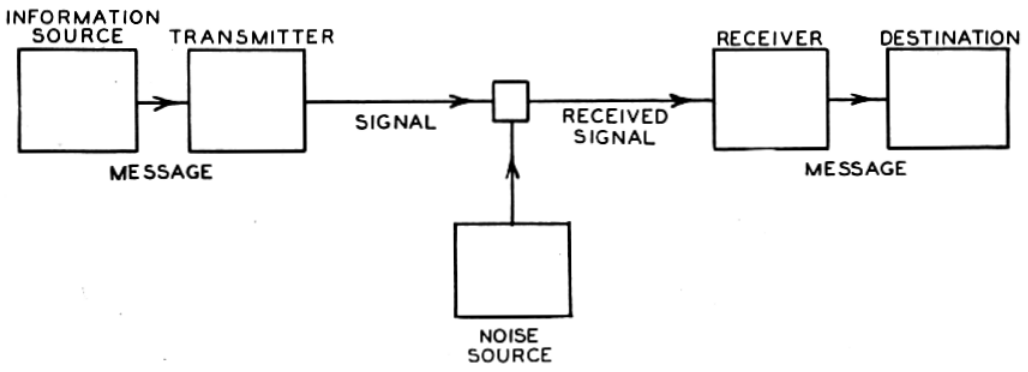
\includegraphics[width=\textwidth]{gfx/03_gesture/ShannonCommunicationSystem.png}
	\caption{Diagramme schématique d'un système général de communication, tel que proposé par Shannon.}
	\label{fig:gesture:shannon}
\end{figure}



Ces deux catégories de geste d'action et de gestes perçu sont emprunt de la théorie de l'information proposée par Shannon \cite{shannon_mathematical_1948} qui envisage la communication comme un système émetteur-message-récepteur unidirectionnel. 
L'inconvenient d'envisager le geste comme simple émetteur d'un signal (qu'il soit travail ou signe) est qu'il empêche de considérer le geste dans la rétroaction dans laquelle il s'inscrit avec l'instrument. En particulier dans la performance musicale, la rétroaction multimodale (par l'ouïe, la vue, le toucher) entre les geste d'un instrumentiste et son instrument, le son et le public est essentielle.

Il était tentant de l'appliquer à la situation musicale et de voir dans le phénomène sonore un message circulant du musicien vers l'auditeur, et les analyses du geste instrumental s'appuyant sur cette solide base théorique ont permis de développer un certain nombre de concept encore utile pour l'analyse du geste musical.

Cependant, la situation de performance musicale est loin d'être aussi fonctionnelle que celle qui consiste à vouloir transmettre un flux de données. Notamment, la théorie de l'information s'applique à des machines qui ignore totalement le contenu sémantique de ces données et les aspects cognitifs ou les références culturelles des émetteurs et récepteurs.
%-------------------------- Figure : transparence Fels -----------------------
\begin{wrapfigure}[14]{R}{0.5\textwidth}
	\begin{center}
 		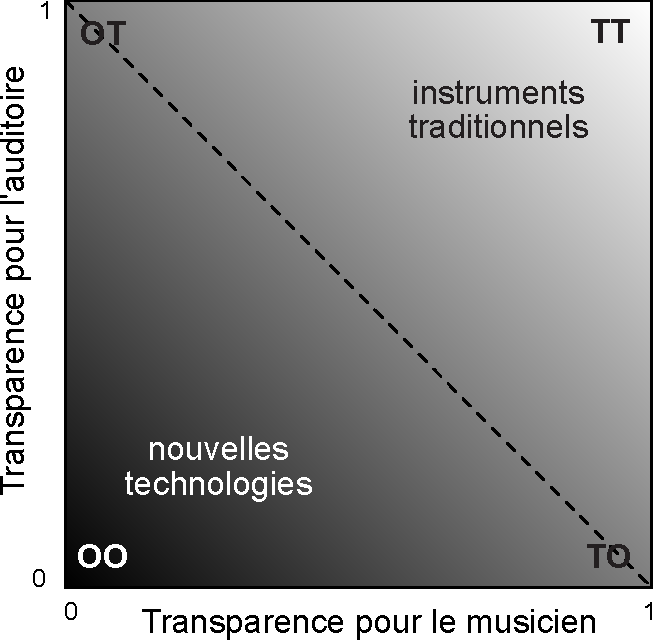
\includegraphics[width=0.48\textwidth]{gfx/03_gesture/Fels-transparency.pdf}
	\end{center}
	\caption{Transparence pour le musicien et l'auditoire, d'après \cite{fels_mapping_2002}}
	\label{fig:gesture:fels_transparency}
\end{wrapfigure}
%-------------------------- Figure : transparence Fels -----------------------

Certains auteurs ont critiqué cette approche \cite{fyans_where_2009} en remarquant que l'idée selon laquelle une connaissance et une compréhension préalable de l'instrument et de l'idiome était nécessaire pour évaluer une performance musicale, ne pouvait être généralisée aux \glspl{DMI}, à cause de l'émergence rapide de technologies, d'instruments et de pratiques de performance dans ce domaine. 

Cependant, cette critique reste ancrée sur une approche qui considère que le spectateur évalue le \textit{succès} d'une performance selon sa compréhension des intentions de l'instrumentiste.


Le jeu musical joue en partie sur l’attente de l’audience (récompensée ou non) sur la base de règles d'harmonies, d’idiomes (e.g. cadences, résolutions, cycles rythmiques), de citations (e.g. via le sampling), etc..
Affordance des instruments ne peut être réduite aux objectifs d’affordance des IHM.


Kurtag Jr. Hangsimotato (video)
Jean Haury Meta-Piano
Applebaum Aphasia

gestes incongruent (Musical gestures, Godoy, p.48)


Charlotte Moorman and Name June Paik performing John Cage’s 26’1.1499” for a String Player (Human Cello section




%%%%%%%%%%%%%%%%%%%%%%%%%%%%%%

1.Introduction

2.Le geste instrumental défini au tournant du siècle
	2.1 Cadoz, Wanderley
	2.2 Influence de la théorie de la communication

3. Les limites d'une analyse en terme de IHM
	3.1 Geste produit, capté, perçu
	3.2 Les musiciens ne sont pas utilisateurs d'instruments
	3.3 La scène et le laboratoire

4. Du geste instrumental au geste musical
	4.1 L'outil comme externalisation chez L-G
	4.2 Le geste programmé (Stiegler et la grammatisation)
	4.3 Le geste de re-sonance

5. Subversion sonore, subversion gestuelle
	5.1 Sons paradoxaux, gestes paradoxaux
		Risset, Kurtag Jr., Kurtag Père
	5.2 Le geste et le son comme métaphores
		5.2.1 Bayle
		5.2.2 UST
	5.3 Continuité artificielles (morphodynamisme des DMI)
		La musique comme jeu de la (dis)continuité

6. Résonance entre le geste re-sonnant et le son

6. Un exemple pratique 



Si le geste est un mouvement accompagné d'intention, il faut prendre en compte cette partie intentionelle et essayer de la qualifier, dans la perspective des conséquences qu'elle porte au design des \glspl{DMI}.

La notion ``d'image de son (i-son)'' de François Bayle exprime la mécanique psycho-poétique de construction de l'œuvre musicale acousmatique. Sa nomenclature ne se prête pas facilement à une application directe dans la lutherie (numérique ou non).
En partant de la classification des fonctions de l'écoute proposée par Pierre Schaeffer et Michel Chion (\cite{chion_guide_1994}, p.26) (Insérer ici le tableau comprendre-écouter-entendre-ouïr), François Bayle retient notamment trois niveaux d'écoute attentive (en regroupant entendre et comprendre dans un seul niveau) qu'il fait correspondre à trois niveau d'intentionalité dans la mise en jeu des \textit{images-de-sons}:
\vspace{-1em}
\begin{itemize}[noitemsep]
\item \textbf{\textit{im-son}}: l'image isomorphe, iconique, référentielle;
\item \textbf{\textit{di-son}}: le diagramme, sélection de contours simplifiés, indiciels ;
\item \textbf{\textit{mé-son}}: la métaphore ou métaforme, reliée à une généralité
\end{itemize}

Ces trois catégories font également écho au catégories de Delalande (gestes effecteurs, gestes accompagnateurs, gestes figurés) — sans qu'il y ait toutefois de relations causales triviales entre ces catégories du gestes et de l'écoute.

%------------------ Bricout: g-son -------------------------
Concept de \textit{g-son} proposé par Bricout \cite{bricout_les_2011}, à partir du concept d'i-son (\textit{image-son}) proposé par Bayle, comme ``dépassement de la suggestion de l'image par le son lui ajoutant de manière beaucoup plus évidente la suggestion du geste, de l'élan physique.''

Romain Bricout : couple ``déclenchement/modulation'' (analogue à l'archétype ``percussion/voix'' Martin Laliberté) comme atomes gestuels constitutif de tout mouvement. => NON tout l'espace gestuel avec toutes les connotations possibles (sémiotiques, mimétiques)

Bricout :
\iquote{Déclenchement et modulation représentent donc ces deux gestes primordiaux, à la base de de n'importe quel autre geste plus complexe. Par voie de conséquence, n'importe quel son renvoie lui-même à un geste producteur qui se rapprochera tantôt du déclenchement, tantôt de la modulation ou, par combinaison, des deux à la fois}
=> qu'en est il d'un field recording ?
%------------------ END Bricout: g-son -------------------------

J'aurais plutôt tendance à employer le terme ``d'image de geste'' (i-geste) pour décrire cette analogie entre les plans d'interprétation du geste et du son.

Le travail de création des correspondances entre geste et son passe ainsi par trois étapes faisant écho à ces différents niveaux de perception/compréhension musicale :
\vspace{-1em}
\begin{itemize}[noitemsep]
\item \textbf{coder} la relation algorithmique (causale ou non), c'est-à-dire concrètement la relation algorthmique qui s'opère entre les signaux captés par l'interface et le contrôle de la synthèse sonore, 
\item\textbf{jouer} la relation sensible, c'est-à-dire pratiquer (chorégraphier) l'ensemble du mouvement gestuel dont une partie seulement sera captée par l'interface de jeu;
\item\textbf{imaginer} la relation poétique, cette relation s'établit sur un ensemble plus complexe de valeurs esthétiques, de références culturelles impliquant de manière plus globale les questions de composition, de scénographie, de métaphores portée par les sons, etc.
\end{itemize}




\subsubsection{Les unités sémiotiques temporelles}

La définition des UST est donnée dans \cite{timsit-berthier_les_2004}:
\iquote{Les UST sont des segments musicaux, qui possèdent une signification temporelle en raison de leur organisation morphologique et cinétique. Elles peuvent êtres considérés comme des représentations iconiques qui entretiennent des rapports de ressemblance avec des modèles temporels naturels. L’UST ne traduit pas le phénomène musical à son niveau acoustique, mais cherche à y trouver en quelque sorte une intentionnalité.}



%%%%%%%%%%%%%%%%%%%%%%%%%%%%%%%%%%%%%%%%%%%%%%%%%%%%%%%%%%%%
%%%%%%%%%%%%%%%%%%%%%%%%%%%%%%%%%%%%%%%%%%%%%%%%%%%%%%%%%%%%
%%%%%%%%%%%%%%%%%%%%%%%%%%%%%%%%%%%%%%%%%%%%%%%%%%%%%%%%%%%%
%%%%%%%%%%%%%%%%%%%%%%%%%%%%%%%%%%%%%%%%%%%%%%%%%%%%%%%%%%%%
%%%%%%%%%%%%%%%%%%%%%%%%%%%%%%%%%%%%%%%%%%%%%%%%%%%%%%%%%%%%
%%%%%%%%%%%%%%%%%%%%%%%%%%%%%%%%%%%%%%%%%%%%%%%%%%%%%%%%%%%%
%%%%%%%%%%%%%%%%%%%%%%%%%%%%%%%%%%
\section*{Espace du geste musical}
La musique a longtemps été considéré comme étant faite d'un sous-ensemble de sons, les sons harmonieux, voire harmonique, avant qu'au \siecle{20}~siècle, les bruits n'y fassent leur place avec les avant-gardes, futuristes. 

John Cage in \cite{cage_silence:_1961}
\begin{quotation}
\noindent If this word, music, is sacred and reserved for eighteenth- and nineteenth-century instruments, we can substitute a more meaningful term: organization of sound.\\
\end{quotation}


Anecdote De Laubier ` le haut parleur ne fonctionne pas'

La musique n'est donc pas faite que de sons, au sens acoustique du terme, mais également (avant tout?) de la perception des sons, qui implique des processus de cognition, des références socio-culturelles, et une sensibilité, une mémoire propre à chacun. 
Ainsi, l'espace de la musique ne se présente non pas comme un sous-ensemble de l'espace des sons, mais probablement comme un sur-espace comprenant à la fois les sons acoustiques mais également tous les liens qu'ils tissent avec notre mémoire.

\Pierre{ voir les 2 définitions de la musique}

L'art musical consiste ainsi à faire entendre des aspects de la musique qui ne sont pas nécessairement présents dans le son, à faire surgir des espaces qui ne peuvent se déployer que dans notre imaginaire, en faisant écho à la trace latente que les sons et la musique ont déjà imprimée en nous.


\begin{quotation}
\noindent Le musical dépasse le sonore en cela qu’il est connecté à une expérience cognitive qui implique la perception et la mémoire.\\
Le sonore dépasse le musical en cela que tout ce qui est sonore ne fait pas nécessairement musique (sauf chez Cage).
\end{quotation}

\Pierre{ ce n'est pas seulement le cas de la musique mais aussi de la parole. Voir définition de Castellengo.}
\Pierre{ Cage -> référence ?}

Là où la présence du musicien sur scène remplissait une nécessité acoustique pour l’écoute, la musique sur support, ou produite par des machines, déplace ce besoin au profit d’une autre fonction, à la fois de compréhension des gestes du musicien (mais est-ce là un jeu de dupes?) et d’un spectacle de l’ordre du funambulisme; le musicien prend des risques [celui de se tromper dans le cas de l’interprétation d’une partition] et la mise en question du corps, réagir au contexte (lieu et au public, ainsi qu’aux éventuels autre musiciens) d’une manière vivante.

L’écoute nous plonge dans des flux sonores, et notre tendance à projeter des causes à ces sons (cf. gestalt) nous emmène sur les lieux — toujours en partie étrangers — de la production de ces flux. sitar indien, crissement de pneu, explosion, acoustique sous-marine ou ambiance de salle de café.
Le musicien crée des passerelles et des agencements entre ces zones liminales.

\Pierre{ si tu parles de gestalt, il faut développer mais c'est aussi une théorie très controversée, donc attention !}

Si les gestes \textit{subversifs} peuvent être assimilés à des gestes accompagnateurs, la plupart des articles de la littérature semble ignorer cette part de subversion au profit de la lisibilité du geste et sa corrélation avec le son \cite{godoy_exploring_2006}.
Cependant, la corrélation n'est pas nécessairement recherchée en tant que telle et si, comme le rappelle Risset, \iquote{la musique est aussi un art du mirage, de l’illusion} \cite{risset_propos_2010}, les œuvres sont nombreuses qui cherchent à dépasser le lien d'apparente causalité entre le geste et le son. 
Il serait alors plus juste d'utiliser le terme de \textit{geste accompagnant la musique}, si toutefois on 

%---- Figure : Einarsson sculpture ---------
\begin{figure}[!htbp]
	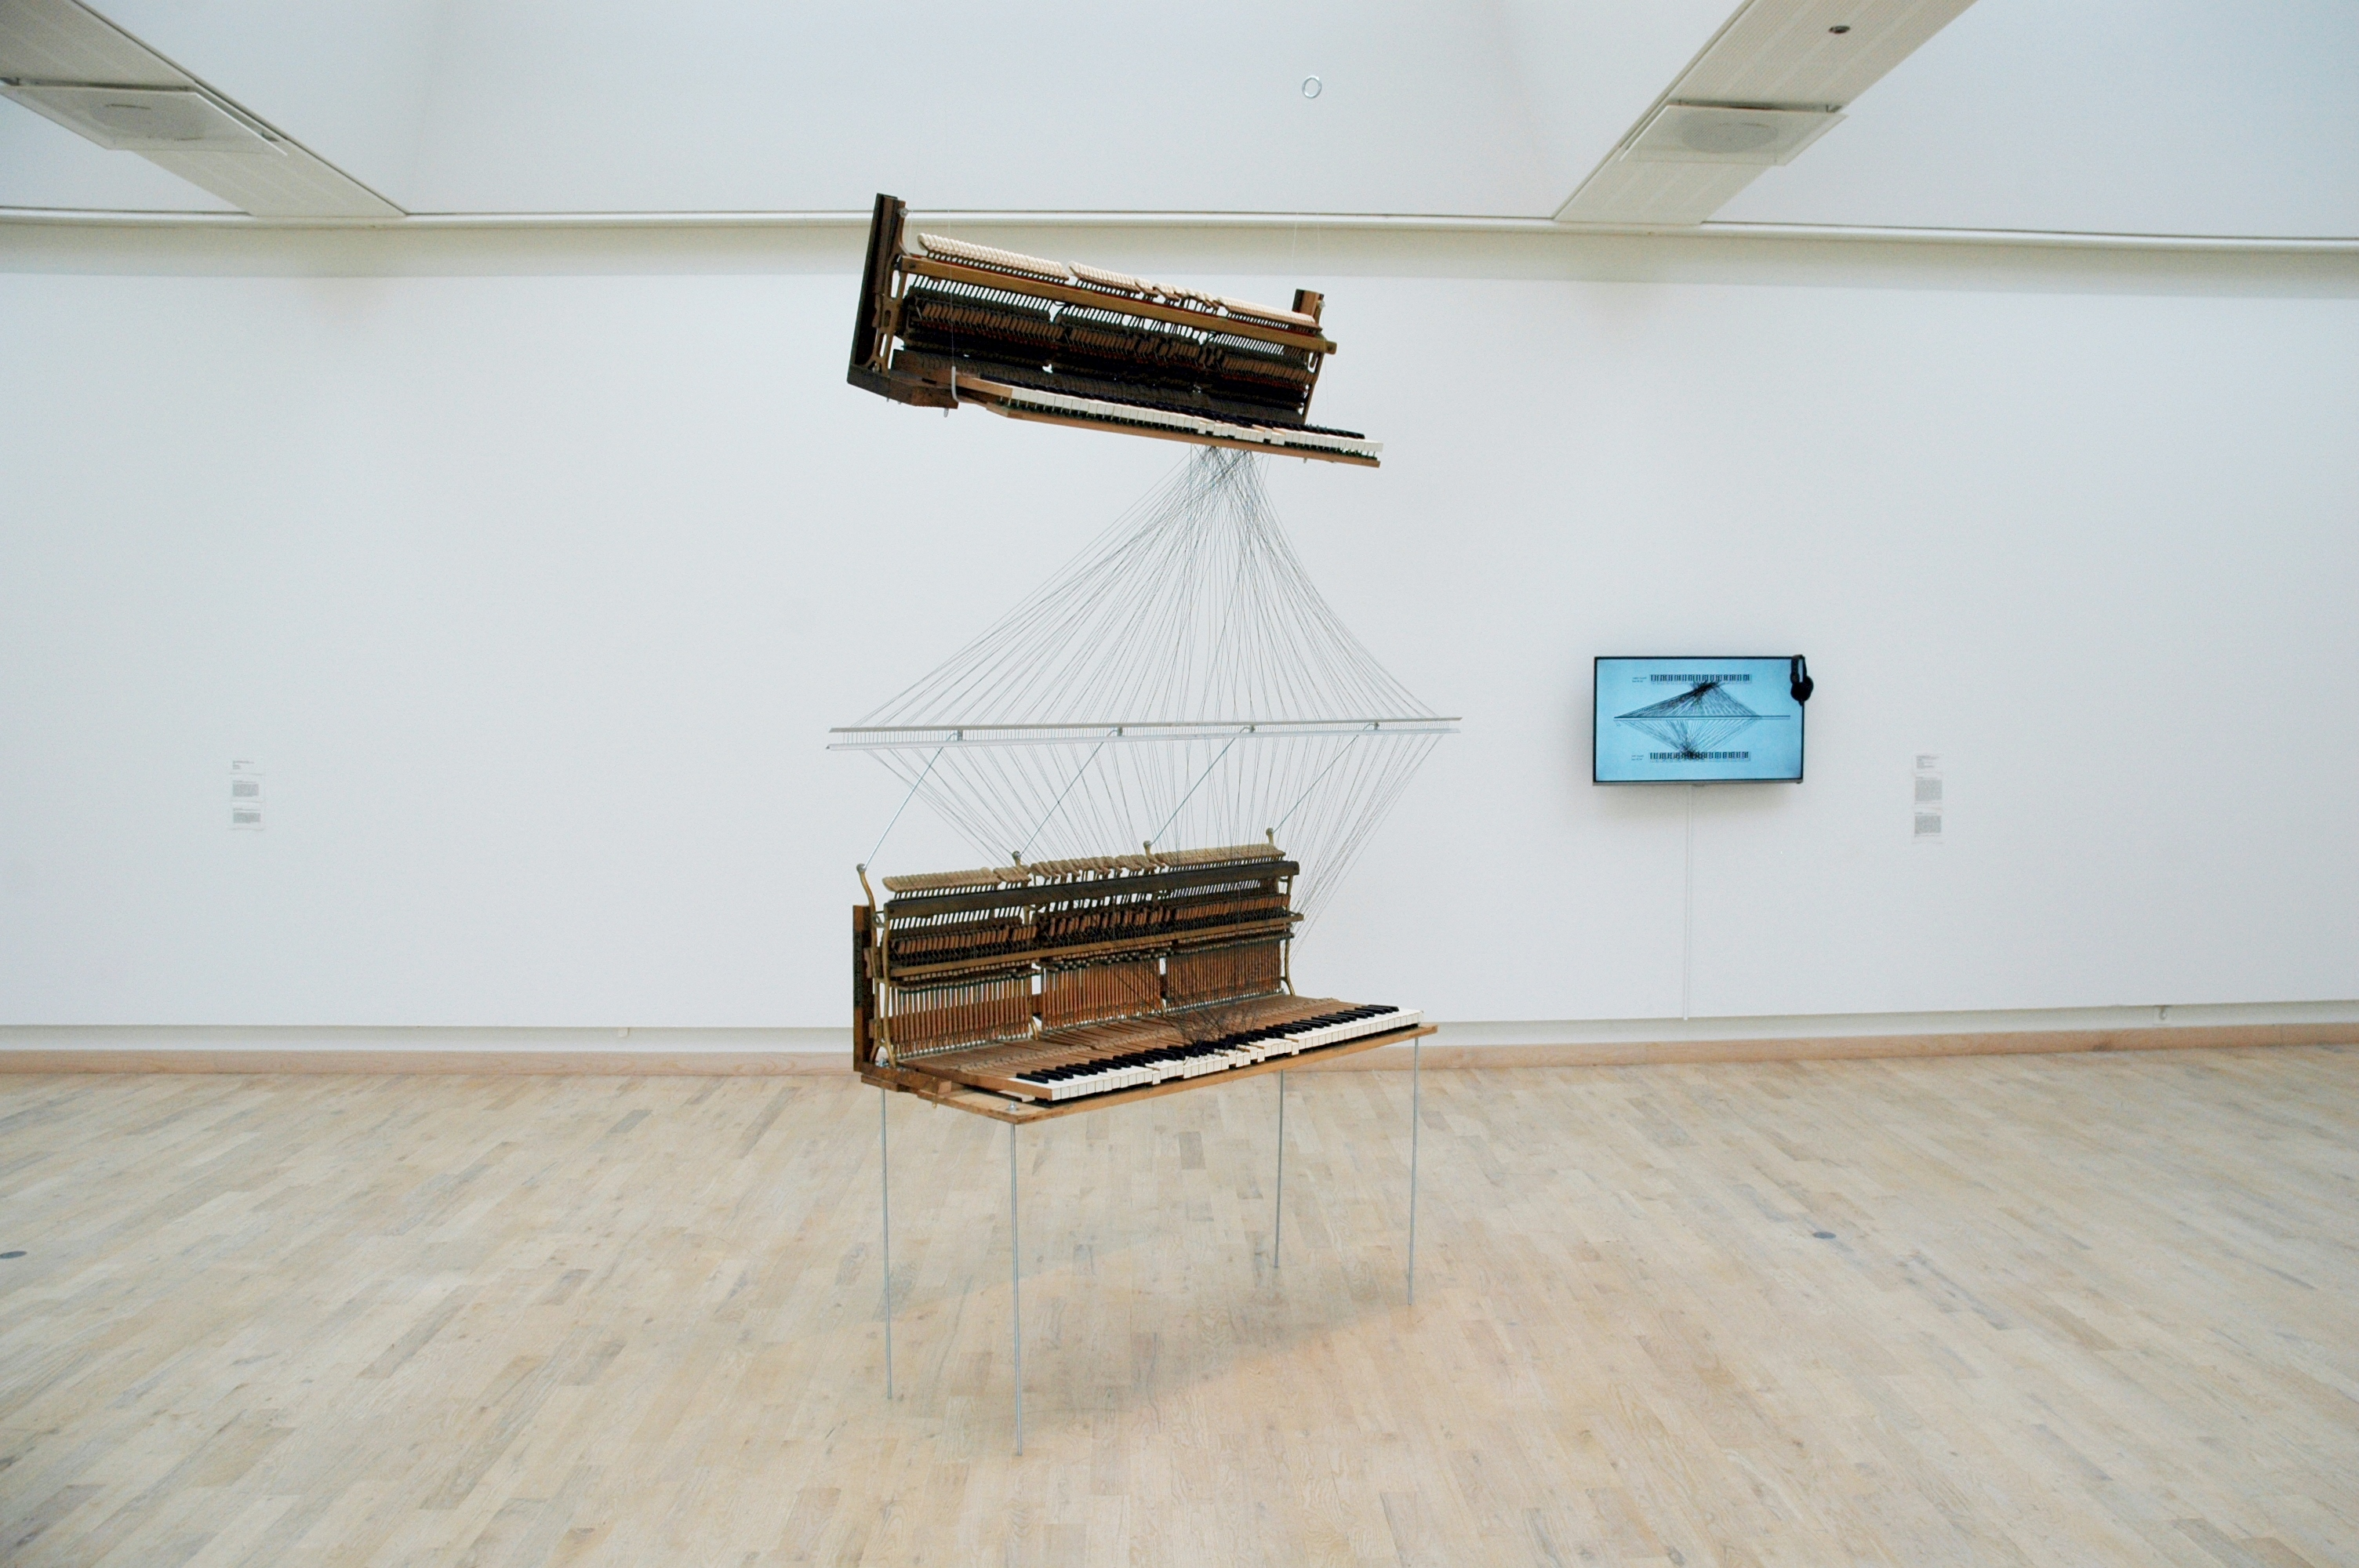
\includegraphics[width=\textwidth]{gfx/Einarson-SchumannSculpture}
	\caption{Einar Torfi Einarsson - Schumann-Sculpture (remnants + deracination)}
	\label{fig:gesture:einarsson}
\end{figure}


\iquote{Every music performance is a dramatic presentation for listeners and improvisers alike. In a sense, both groups play interactive roles as actors from their respective platforms. Just as the design of the hall, the stage and the lighting frames the band's activity for the audience's observation, it also frames the audience's activity for the band to observe. Performers and listeners form a communication loop in which the ction of each continuously affect the other.} Paul F. Berliner in \cite{berliner_thinking_2009}


%%%%%%%%%%%%%%%%%%%%
%-------------------------------------------
\subsection*{Dans les instruments numériques}


Les \glspl{DMI} ont souvent été analysés en tant qu'\gls{IHM}, et les conférences académiques qui leur sont consacré reflètent une culture dans laquelle l'interaction s'exprime via un cahier des charges préalablement identifié: une \gls{IHM} est utilisée dans le cas d'une tâche précise et sa qualité (ergonomie, précision, etc.) peut être mesurée de manière quantifiée.
Dans le cas des instruments de musique cependant, cette tâche est plus complexe, car les enjeux de la création musicale dépassent par essence tout objectif identifié et mesurable au préalable. Par ailleurs, les \glspl{DMI} sont destinés à plusieurs types "d'utilisateurs" ayant un rôle différent : le musicien qui joue de l'instrument, mais également le public, qui bien qu'il ne joue pas de l'instrument est amené à en observer la performance.

Low entry fee, high ceiling.

La performance musicale est un "jeu" qui comporte une part de duplicité. Le public d'un concert est toujours le sujet d'une illusion. 

Un des biais de la littérature sur l’affordance des instruments de musique numérique est qu’elle s’inspire souvent des objectifs de l’affordance des IHM en général, avec l’idée que l’instrument doit être compréhensible pour les “autres” utilisateurs potentiels que l’auteur de l’instrument. Pourtant, nombre d’instruments présentés dans la communauté NIME ne sont joués que par leurs auteurs (cf. [1], [2], [3]) et si le fait de vouloir transmettre son instrument aux autres est louable, il n’est pas gage de qualité en ce qui concerne la création qui sera faite avec cet instrument. 


L'art musical procède en partie de la magie et de l'illusion perceptive. Le musicien nous fait entendre des continuités (e.g. une mélodie) là où l'acoustique fait apparaitre une série discrète (e.g. des notes de piano), ou inversement des fissions (e.g. deux voix indépendantes) là où est jouée une série temporelle de notes sur un même instrument. (=> plutôt que des exemple entre parenthèse, mettre une figure illustrant fission e.g. Bach's Violin Partita No. 3, BWV 1006.)

Cette question du jeu entre le continu et le discret dépasse le seul cadre de la musique mais semble trouver dans cet art de nombreuses espaces d'expression.

Les théories de la perception, en particulier du Gestalt, viennent en partie expliquer les mécanismes qui pousse notre perception à créer des continuités où il n'en existe pas physiquement et inversement à catégoriser des événements selon certaines distances perceptives qui ne sont pas nécessairement en lien avec l'unité de source de production du son.

Si donc on analyse le geste musical, il faut nécessairement prendre en compte sa dimension subversive en ce qu'elle se traduit, particulièrement dans le cas des \glspl{DMI} et des productions musicales impliquant l'électronique en général, dans le design des instruments et outils qui servent à la créer.

\cite{bin_show_2018}

Une étude de Tsay \cite{tsay_sight_2013}, dans laquelle des amateurs et experts sont amenés à évaluer une performance musicale sur la seule base d'un enregistrement silencieux, met en évidence le rôle considérable du la part visuelle dans l'appréciation et l'évaluation de la performance.

Carte et guide , frettage adaptatif (cite \cite{goudard_playing_2014})


\iquote{De même, pour un violoniste, la manière dont il lève le bras et dont il va attaquer le son, la rapidité avec laquelle il prépare son coup d’archet nous renseignent un petit peu, mais pas complètement – parce que l’on ne sait pas quelle hauteur il va jouer – sur certaines catégories du son, comme le fait que le son sera agressif, fort, ou délicat et très doux. (...) Dans la musique instrumentale, cette causalité est très importante car cela participe de la façon dont nous la percevons et l’intérêt, avec la musique électronique, c’est que l’on peut remettre en question cette causalité-là : un tout petit geste peut provoquer une tempête. Entre le geste du pianiste qui va appuyer sur une touche du piano et le son qui va sortir, il y a une machine que j’appelle une boîte noire, qui peut inverser les polarités, c’est-à-dire que je peux très bien programmer la machine de manière à ce que plus le son qui va être joué va être minime, pianissimo, plus le son électronique qui va sortir va être au contraire démesuré : dans ce cas-là, le geste ne correspondra pas du tout au son.} Philippe Manoury interviewé par Anne-Sylvie Barthel-Calvet. (\url{https://geste.hypotheses.org/364})

Dans en Echo de Manoury, ce sont les formants de la voir qui contrôlent la partie électronique, c'est-à-dire un geste invisible, sans contact. (extensible au suivi de partition)


Pouvoir transformer tout type de donnée en geste programmé.


L'interface sensible\footnote{Sur la notion d'interface sensible, cf. \ref{ch:interfaces}} doit pouvoir se prêter à des gestes sans intention, c'est-à-dire qu'elle doit permettre des gestes non-réfléchi, mal-contrôlé ou plutôt in-controlés, qui peuvent tomber en dehors de la zone prévue pour capter de le geste, où d'une manière inadéquate. Cela ne signifie pas nécessairement que l'instrument doit ``faire quelque chose'' de ces gestes: il peut les ignorer.  Mais il est utile que l'intrument permette aux gestes de ``déborder'' du cadre prévu pour leur interaction (si toutefois ce cadre existe).


%-------------------------------------------
\subsection*{Tout ce qui bouge n'est pas geste - partie à revoir ou distribuer}

Dans le domaine de la recherche musicale, les mouvements du corps sont associés à la notion de \textit{geste musical}, c'est-à-dire à un concept associant à la fois le \textit{mouvement} du corps et \textit{l'intention} et/ou \textit{la signification} de ce mouvement. 

Cela n'est pas nécessairement et systématiquement le cas et les mouvements de l'instrumentiste peuvent être envisagés et décrits avec d'autres perspectives que celle de leur potentielle intention. \todo{ref ou footnote ici vers des études en ce sens} La notion de \textit{geste musical} semble en effet implicitement suggérer un rapport hiérarchique entre le musicien et son instrument, dans lequel les gestes ne serait produits qu'intentionnellement, à l'initiative du musicien. Les instruments de musique, et en particulier les DMIs, sont envisagés plus récemment comme \textit{agents} qui opèrent dans un système de relations multi-directionnelles\todo{ref}, que Berliner décrit métaphoriquement par une \textit{conversation} dans \cite{berliner_thinking_2009}. \todo{attention,il parle de la relation musicien/public} 

\Pierre{ je doute qu'il y ait beaucoup de gestes non-intentionnels chez le musicien !}


Les gestes du musicien ne sont pas nécessairement remplis d'une intention ou d'une signification \textit{a priori}, ils peuvent s'apparenter aux gestes de la danse.




L'instrument vibre et produit parfois du son sans qu'il soit explicitement déclenché ou controlé. Les mouvements du corps du musicien en témoignent et au dela des effets spectaculaires des DJs qui touchent aux potentiomètres de leurs interfaces comme s'ils étaient brûlants \footnote{Mark J. Butler apelle \iquote{passion of the knob} (\textit{la fièvre du potentiomètre}) ces moments qui surviennent \iquote{lorsqu'un musicien dirige une expressivité exceptionnellement intense vers un petit composante technique associée à l'ingénierie du son} \cite{butler_playing_2014} \url{https://www.youtube.com/watch?v=Nh9C7nQHmII}}, le corps est parcouru de mouvements qui ne sont pas uniquement des \textit{actions} mais des \textit{réactions} à ce qui est produit par l'instrument. 

\Pierre{ l'exemple choisi devrait être un peu plus analyser car les mouvements du DJs sont probablement totalement intentionnels - c-a-d ils font partie du spectacle car le DJ se sait regardé.}
\Pierre{ je crois plus en la séparation geste-signe et geste-action}

Si l'on considère la relation geste/instrument/musique comme un réseau multi-directionnel, le geste peut-être provoqué par la musique, via l'instrument lui même. Deux exemples caricaturaux viennent illuster cette possibilité : la performance \iquote{eletric stimulus to face — test} de l'artiste Daito Manabe\footnote{\url{http://www.daito.ws/work/electricstimulustoface_test.html}} ou dans le système de motorisation des doigts pour apprendre un instrument proposé récemment à la conférence NIME par \cite{zhang_adaptive_2019}.


Notons enfin que les mouvements peuvent survenir également en interaction avec le public\footnote{This reveals that passion-of-the-knob moments and other actions are not interior to the musician’s world, but rather are intensely meaningful communications: they reverberate outward to the audience and then are reflected back to the stage as formative elements of a milieu whose participants seek to actively cultivate and sustain liveness. in \cite{butler_playing_2014}} 



\subsection*{geste d'impression, geste d'expression}
Si le geste peut ex-primer, c'est-à-dire ``faire sortir en pressant'', un mouvement intérieur et le faire exister dans la temporalité de la performance, il peut aussi im-primer (faire rentrer, en pressant) ce geste sur un support à même d'en accueillir la trace.

geste du latin gero qui signifie ``porter''

S'il y a différance (ajournement et différence) dans la grammatisation musicale (la composition, la lutherie, la programmation), il y a enfin le moment de sa performance, de sa répétition.

Classification des controleurs gestuels dans \cite{wanderley_controgestuel_1999}:
\vspace{-1em}
\begin{itemize}[noitemsep]
\item \textbf{Instrument-like controllers},where the input device design tends to reproduce each feature of an existing (acoustic) instrument in detail. Many examples can be cited, such as electronic keyboards, guitars, saxophones, marimbas, and so on.
\item \textbf{Instrument-inspired controllers} that although largely inspired by the existing instrument’s design, are conceived for another use [62]. Fig. 3 presents one example of such controller, the SuperPolm violin developed by S. Goto, A. Terrier, and P. Pierrot [63], [64], where the input device is loosely based on a violin shape, but is used as a general device to control granular synthesis. => emprunts variés de formes et de fonctions.
\item \textbf{Extended instruments} are instruments augmented by the addition of extra sensors [58], [65]. Commercial augmented instruments included the Yamaha Disklavier, used, for instance, in pieces by J.-C. Risset[66], [67]. Other examples include the flute [68]–[70] and the trumpet [71]–[73], but any existing acoustic instrument may be extended to different degrees by the addition of sensors.
\item \textbf{Alternate controllers} (see, e.g., Fig. 4), whose design does not follow that of an established instrument. Some examples include the Hands [52], graphic drawing tablets [74] (cf. Fig. 5), etc. For instance, an unorthodox gestural controller using the shape of the oral cavity has been proposed in [75].
\end{itemize}

These controllers can furthermore be classified into different categories.
\begin{itemize}[noitemsep]
\item \textbf{Touch, expanded range, or immersive} controllers [76], depending on the amount of physical contact required from the performer. Mulder also [76] separates immersive controllers into internal, external, and symbolic controllers according to the possibilities of visualization of the control surface. In a different approach, Piringer [77] classifies immmersive controllers into partial or completely immersive controllers.
\item \textbf{Individual or collaborativecontrollers}[78],depending on whether the instrument is performed by one or multiple performers at one time.
\item \textbf{Metaphorical} or \item{ad hoc} controllers, and so on.
\end{itemize}


Guerino Mazzola frozen gestures



\iquote{Complétons tout d’abord la phrase : l’ordinateur n’est pas un instrument mais une représentation d’instrument. Cette subtile nuance contient l’essentiel. Envisagé ainsi, l’ordinateur donne une nouvelle dimension au processus de création en y intégrant explicitement, en amont de l’acte instrumental, la construction d’une représentation du dispositif instrumental. Cette construction\/représentation offre une latitude nouvelle : la possibilité pour l’homme de se placer dans une relation ``de type instrumental'', une représentation de relation instrumentale où la liberté d’échapper aux contingences du réel lui permet de créer de nouveaux mondes imaginaires. 
Toutefois, le processus de création est également considérablement transformé par le fait que l’aller\/retour indispensable entre le réel et l’imaginaire, lui aussi, se déplace. Dans le cas de l’instrument réel, l’aller\/retour se fait in situ, dans la relation même avec l’instrument. Dans le cas de la représentation d’instrument, il se fait dans une boucle plus vaste : l’activité de représentation instrumentale, de jeu virtuel, de composition façonnent nos sens et notre intelligence d’une nouvelle manière qui sont alors en jeu dans une perception nouvelle du monde réel... à condition que nous y retournions, c’est à dire que nous ne finissions pas par substituer définitivement nos représentations à la réalité.} \cite{cadoz_musique_1999}, p99.

Claude Cadoz défend l'hypothèse que les appareils électroniques ne sont pas des instruments mais des ``représentations d'instrument''.


